\documentclass[journal]{IEEEtran}
\usepackage[T1]{fontenc}
\usepackage{graphicx}
\usepackage{booktabs}
\usepackage{amsmath}
\usepackage{array}
\usepackage{longtable}
\usepackage{tabularx}
\usepackage{enumitem}
\usepackage[hidelinks]{hyperref}
\usepackage{url}
\graphicspath{{../figures/}}
\newcommand{\figplace}[2]{\IfFileExists{figures/#1.png}{\includegraphics[width=\linewidth]{#1}}{\fbox{\parbox[c][0.22\textheight][c]{0.94\linewidth}{\centering #2}}}}
\newcolumntype{Y}{>{\raggedright\arraybackslash}X}
\begin{document}
\title{Multi-View and Multimodal Perception for Class-Wise Fruit Inventories: A Design-Space Review}
\author{Muhammad~Zainal~Muttaqin and Fatma~Indriani%
\thanks{Department of Computer Science, Universitas Lambung Mangkurat, Banjarbaru, Indonesia.}}
\maketitle
\begin{abstract}
A class-wise fruit inventory must turn repeated photographs of a plant into
one record for each physical fruit. In the SawitMVC oil-palm dataset, 18,540
annotated boxes depict 9,823 bunches, and a naive sum of even correct boxes places
all four class counts within one bunch of the truth on only 6.38\% of test trees. This design-space
review follows a detection from the image to the inventory, with oil-palm
fresh-fruit bunches as the principal case and mechanisms drawn from tracking,
re-identification, multi-view geometry, and multimodal perception. It defines
six identity mechanisms, from intra-view counting and statistical correction to
appearance matching, temporal tracking, geometric association, and learned
multi-view association, and ties each to the acquisition assumptions it needs.
Orchard studies from 2016 to 2026 supply a measured failure for each mechanism:
calibration cannot name the duplicated fruit, appearance descriptors did not
improve tracking of look-alike fruit, monocular reconstruction lacks scale and
lost fruit when two sides of a tree were joined, and metric SLAM admitted
duplicates where pose drift exceeded the spacing between fruit. The detector
literature explains how instances form under crowding and why one-to-one
assignment within an image does not extend across images. Depth is a
conditional aid for small and occluded bunches whose value depends on its
physical meaning, registration, and quality control; the fusion literature
agrees on quality gating but disagrees on where depth should enter. Direct
oil-palm evidence covers detection, ripeness, and single-bunch grading, but
not cross-view deduplication with depth. The review defines the measurements
needed to test duplicate-aware, class-wise inventories under field conditions.
\end{abstract}
\begin{IEEEkeywords}
multi-view perception, multimodal fusion, object detection, fruit counting,
instance identity, oil palm, design-space review
\end{IEEEkeywords}
% v3: narrative revision. Each section opens from a documented failure case and
% hands its unresolved part to the next section. Appendices are unchanged from v2.
\section{Introduction}

The SawitMVC dataset makes the central difficulty of fruit inventory measurable. Its 3{,}992 smartphone images show 953 oil-palm trees photographed from four or eight positions around the trunk, and its annotators drew 18{,}540 bounding boxes. Those boxes depict 9{,}823 physical bunches. Each bunch appears in one to six views, 74.6\% of them appear in at least two, and the mean appearance count is 1.89 \cite{indriani2026sawitmvc}. The baselines published with the dataset show what this duplication does to a count. When the ground-truth boxes of a tree are summed, the count of a maturity class is within one bunch of the truth for 50.00\% of the class-and-tree cases, and all four classes are within one bunch at the same time for only 6.38\% of the 141 test trees. Dividing the sum by the duplication ratio of the training split ($k=1.89$) raises the two figures to 95.57\% and 86.52\%, and a support-vector regressor on cross-view count features reaches 96.81\% and 88.65\%. The same two counters, when they receive boxes from a YOLO26m detector with a test AP50 of 0.531 (0.354 for the least mature class), fall to 72.34--75.35\% and 30.50--33.33\% \cite{indriani2026sawitmvc}.

The table records two different failures. The first is duplication. A correct detection of a bunch in a second photograph adds a second unit to the count unless some step decides that both observations show the same object. The second is detection. A counter that is almost exact on annotated boxes loses more than half of its tree-level accuracy when it receives predicted boxes. A per-image detection score measures the second failure only. It contains no information about the first.

The problem is older than the oil-palm case. In 2016, Stein \textit{et al.}\ scanned 522 mango trees carrying 71{,}609 fruit from a ground vehicle and compared three ways of counting them: one image per tree, two opposing images, and a multi-view method that followed each fruit between frames with the vehicle's navigation data and triangulated it in 3D \cite{ledger_r_408d13511cac4177}. Against 16 hand-harvested trees, the single-view count followed the harvest count closely but recovered only part of it. Its regression slope was 0.54, so the estimate was usable only after calibration against hand counts. The multi-view count had a slope of 1.014 and an error of 1.36\% per tree without any calibration. The single view was nevertheless the more repeatable of the two ($R^2=0.96$ against 0.84), and the authors observed that the multi-view pipeline, being more complex, had more ways to fail. The choice between a statistical correction that is stable but blind to individual fruit, and an explicit identity mechanism that is accurate but fragile, returns in almost every study examined below. SawitMVC reproduces it for oil palm: dividing by $k$ is a statistical correction, and the cross-view identity links distributed with the dataset make the explicit alternative testable.

Oil palm makes both routes harder than mango. Bunches change sharply in apparent size with camera distance and viewing angle. Fronds and neighbouring bunches hide them partly or completely, and the canopy mixes deep shadow with direct sunlight. The least mature bunches are dark and close in colour to the surrounding fronds. RGB appearance remains necessary for the colour and texture cues that separate maturity stages, but it becomes ambiguous where foliage, shadow, and fruit share local appearance. A detector that ranks well on a generic RGB benchmark has not yet shown that it separates crowded bunches, keeps an identity across views, or survives the failure of an outdoor sensor.

This review follows one detection from the image to the inventory and asks, at each step, what evidence shows that the step preserves the identity of the physical fruit. Section~\ref{sec:designspace} defines the steps and six identity mechanisms (M0--M5), each tied to the acquisition assumptions it needs. Section~\ref{sec:instance} examines how detectors form instances under crowding and scale variation, and why uniqueness inside one image does not extend to a second image. Section~\ref{sec:identity} begins with the orchard studies that measured double counting directly, then traces the tracking, camera-pose, depth, and 3D methods that those studies borrowed or now need. Section~\ref{sec:multimodal} examines when depth and other modalities help and what the direct oil-palm evidence currently supports. Section~\ref{sec:synthesis} returns to the failures recorded in the orchard studies and states which of them the literature has resolved.

The scope is agricultural fruit perception, with oil-palm fresh-fruit bunches (FFB) as the principal case. Mechanisms from tracking, re-identification, multi-view detection, structure from motion, and multimodal perception are treated as transferable evidence, not as agricultural performance claims. Classification is treated as an attribute of an instance. Maturity is the motivating case, but a per-class inventory is undefined until the instance that carries each label has been identified. Previous reviews organize this literature by sensor, ripeness, detector family, or agricultural application; this review takes the cross-view identity of each physical fruit as its organizing variable. Its contributions are threefold: (1)~a six-mechanism taxonomy (M0--M5) for duplicate control under explicit acquisition assumptions; (2)~a comparative synthesis of detector, geometry, fusion, and association evidence according to the decision each mechanism supports; and (3)~an agricultural interpretation that separates direct evidence from transferable mechanisms and identifies the measurements required for a duplicate-aware, class-wise inventory. Table~\ref{tab:position} states the positioning against six earlier reviews, and Figure~\ref{fig:taksonomi} places the questions in one decision space.

\begin{figure*}[t]
\centering
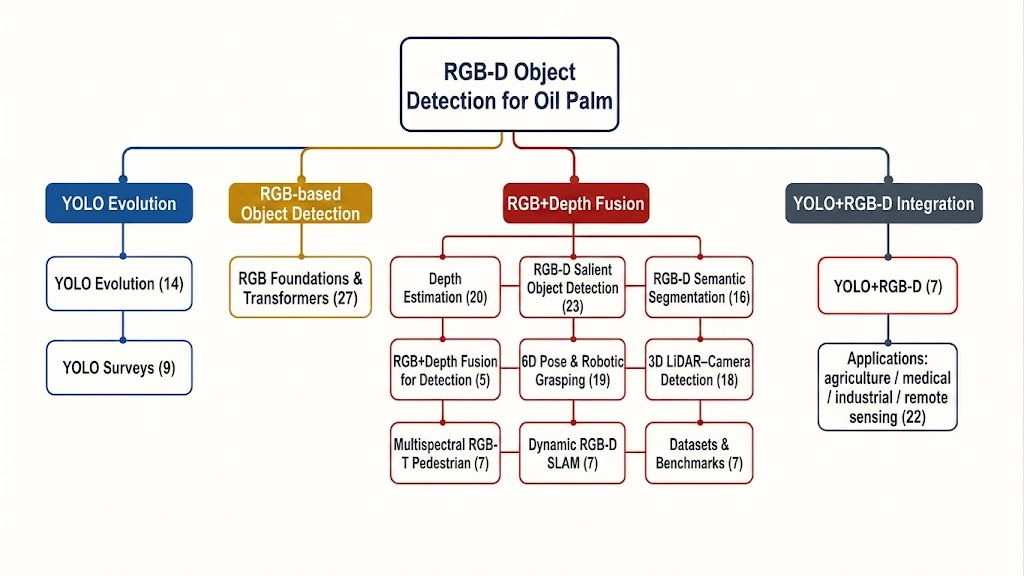
\includegraphics[width=\linewidth]{F01-taksonomi-gpt-image-2-en}
\caption{Conceptual map of the review. The FFB perception problem is decomposed along four axes: RGB detection, depth, RGB-D fusion, and geometry/association, each supported by a cluster of the reviewed literature. A single work may belong to more than one cluster, so the cluster sizes are not additive.}
\label{fig:taksonomi}
\end{figure*}


\section{Review approach and evidence interpretation}

This article is a structured evidence-mapping review. Its purpose is to compare the mechanisms that support class-wise fruit inventories, not to estimate a pooled effect or to rank all models on one benchmark. The synthesis draws on primary literature across object detection, depth estimation, RGB-D fusion, three-dimensional perception, temporal association, and agricultural fruit systems. A reproducible update search used Scopus and OpenAlex for publications from 2015--2026; exact queries, search counts, and screening records are provided in Appendices~B and~C and the supplementary exports.

Studies were retained for the focused evidence register when they provided verifiable full text, a per-instance visual task, an identifiable dataset or acquisition protocol, and a quantitative evaluation. Duplicate records were resolved primarily by normalized DOI and otherwise by normalized title plus year, with conflicts retained for manual review. The complete eligibility rules and selection trace are reported in Appendix~C.

The interpretation rule is more important than the retrieval sequence. Direct evidence comes from agricultural or fruit studies and can support claims about a related deployment setting. Transferable evidence comes from another domain but tests a mechanism-level question, such as whether geometry preserves identity or whether fusion resists missing depth. Design hypotheses specify what should be tested for FFB perception and are not presented as achieved agricultural results. This boundary prevents evidence from indoor RGB-D, autonomous driving, or generic detection from being read as proof of field performance.

\section{Design space for unique class-wise inventories}
\label{sec:designspace}

\subsection{From detections to inventory}

The task has five distinct operations. First, a detector or segmenter proposes an instance in each observation. Second, a class head attaches an attribute to that instance. Third, observations are associated when they refer to the same physical object. Fourth, duplicate observations are rejected or merged. Fifth, the remaining identities are aggregated into counts per class. The first two operations can be evaluated with precision, recall, average precision, and class confusion. The last three require identity and count metrics.

This decomposition changes the interpretation of a strong detector. A detector with high average precision on independent images may still overcount when a tree is filmed from both sides. A tracker may preserve identity through a short video but fail when the camera returns after a gap. A 3D association method may remove duplicates but become unusable when depth is uncalibrated. The design choice is therefore conditional on the acquisition regime.

\subsection{Six identity mechanisms}

Table~\ref{tab:mechanisms} defines the six mechanisms used in the synthesis.

\begin{table}[t]
\centering
\caption{Identity mechanisms and their minimum assumptions.}
\label{tab:mechanisms}
\small
\begin{tabularx}{\columnwidth}{@{}lY Y@{}}
\toprule
Code & Mechanism & Main assumption and risk\\
\midrule
M0 & Intra-view detection or segmentation & One view is sufficient. Hidden objects and repeated views are not resolved.\\
M1 & Statistical correction or fixed census & Duplicate structure is stable enough for a correction factor. The correction may not transfer across trees.\\
M2 & Appearance or re-identification & The instance retains discriminative texture, colour, or shape despite illumination and occlusion.\\
M3 & Temporal tracking & Consecutive observations overlap in time and motion is sufficiently smooth. Track fragmentation and drift remain possible.\\
M4 & Geometric or 3D association & Calibration, scale, or reliable reconstruction is available. Sensor failure and SfM cost are risks.\\
M5 & Learned multi-view association & Linked training data represent view, class, and occlusion variation. The model may overfit one acquisition pattern.\\
\bottomrule
\end{tabularx}
\end{table}

M0 is the no-association baseline. M1 uses a statistical correction or a fixed counting protocol without assigning a persistent identity. M2 matches local appearance or a learned re-identification embedding. M3 uses temporal continuity, motion, and track management. M4 uses calibrated geometry, depth, SfM, or a 3D map. M5 learns a multi-view association function directly from linked observations. A system can combine mechanisms, but its reported result must identify which mechanism is responsible for duplicate rejection.

Every mechanism in Table~\ref{tab:mechanisms} has at least one agricultural study in which it was built, measured, and found to fail in a specific way; Section~\ref{sec:identity} examines them in order. M1 is the division by $k$ in SawitMVC and the harvest-calibrated correction that turned MangoYOLO detections into orchard load estimates \cite{indriani2026sawitmvc,koirala2019deepfruit}. M2 is the appearance descriptor of DeepSORT, which did not improve apple tracking over a tracker that used motion alone \cite{ledger_r_2d972b94554c6cd1}. M3 is the motion-based tracking with a fixed counting region that Zhang \textit{et al.}\ used for citrus \cite{ledger_r_ee550a3e3a6fb318}. M4 is the structure-from-motion or SLAM step that removed double-counted tracks in orange, mango, and pear orchards, and that in the pear orchard still admitted 53 duplicates \cite{ledger_m_9966d81433d61ed3,ledger_r_00f82e0f404d691b,ledger_r_d4270ea8ab11f268}. M5 is the learned descriptor matching that Fusaro \textit{et al.}\ trained to re-identify strawberries between scans taken at different dates \cite{ledger_r_0eda6374aaf85fae}.


\subsection{Acquisition assumptions}

The second design axis is the assumption set. A1~is the amount of overlap and occlusion. A2~is the camera baseline or view separation. A3~is motion smoothness or scene stationarity. A4~is calibration and metric scale. A5~is appearance distinctiveness. A6~is regularity of duplicate exposure, for example a fixed four-side census. A7~is the availability of identity supervision or an oracle association. M1~mainly depends on A6. M2~depends on A5. M3~depends on A3. M4~depends on A2 and A4. M5~depends on A7 and on coverage of the training acquisition pattern.

This two-axis view gives a precise meaning to the phrase ``multi-view deduplication.'' It is not a mandatory module. It is a mechanism whose value should be tested against the assumptions that survive in the field. A fixed four-side protocol may make M1 competitive when duplication is regular and metric depth is unreliable. An unstructured moving camera may require M3 or M4 because the number and order of observations are not fixed.

\subsection{Class attributes beyond maturity}

Maturity classification is common in FFB literature, but the identity dependency is more general. An instance may carry a maturity label, a size class, a defect label, a disease state, a variety label, or a harvest-readiness state; oil-palm mills, for example, must distinguish Dura from Tenera bunches, which differ in fruitlet density and surface intensity \cite{ledger_r_722bfce242f37ecb}. The inventory should first establish one identity record and then attach one or more attributes to that record. If the same bunch appears in three views with two maturity predictions, the system must report whether the conflict is resolved by confidence, temporal evidence, geometry, or manual adjudication. Summing per-view class predictions without this step is not a class-wise inventory.



\section{Evidence for instance formation and class attribution}
\label{sec:instance}

The detector literature is used as decision evidence. The relevant question is which architectural properties preserve instances under crowding, scale variation, latency constraints, and class confusion in field imagery.

\begin{figure*}[t]
\centering
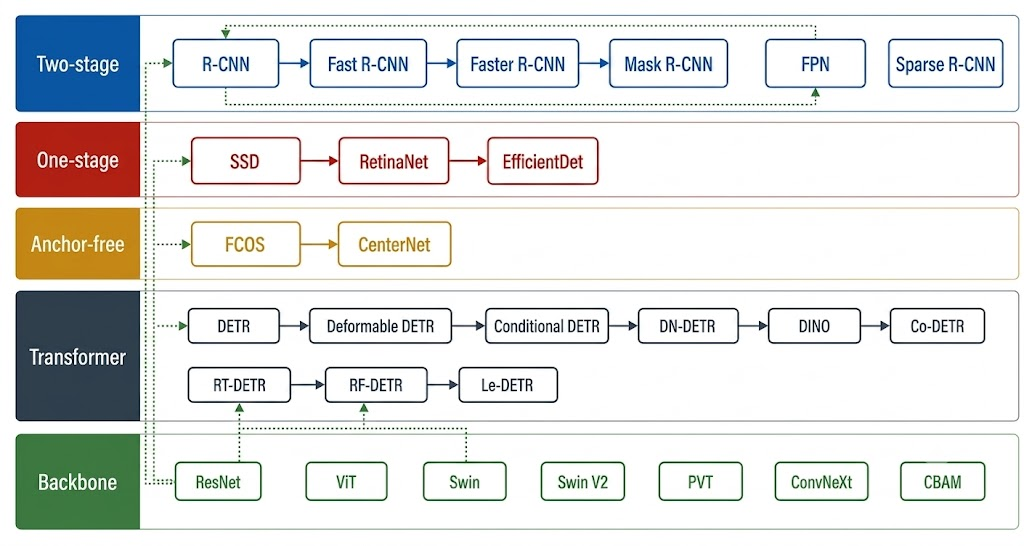
\includegraphics[width=\linewidth]{F03-silsilah-rgb-gpt-image-2-en}
\caption{Genealogy of the RGB detector paradigms and the inheritance of ideas between them: the two-stage line (R-CNN through Sparse R-CNN), the one-stage line (SSD, RetinaNet, EfficientDet), the anchor-free line (FCOS, CenterNet), and the transformer line (DETR through the real-time DETR variants).}
\label{fig:silsilah}
\end{figure*}

Across RGB detector families, recurring responses to localization, scale, class imbalance, and computational cost define the choices relevant to fruit inventory. Zou \textit{et al.} synthesize the corresponding one- and two-stage families \cite{zou2023objectdetectionsurvey}. Figure~\ref{fig:silsilah} maps four detector paradigms and their design relationships as supporting context for the comparisons below. Because these detectors were validated on generic benchmarks, they enter this review as baseline and mechanism evidence, not as FFB performance claims.

\subsection{Instance separation under crowding and scale}

The deep-detection era opens with R-CNN, whose central move was to separate the localization problem from the recognition problem. Instead of sliding a classifier across every position and scale, R-CNN accepts a few thousand class-agnostic region proposals produced by a bottom-up algorithm and runs a convolutional network only inside each proposal; localization is delegated to the proposal generator, and the network's job is reduced to recognizing the contents of a given region \cite{girshick2014rcnn}. This yielded 53.3\% mAP on PASCAL VOC 2012, a relative improvement of more than 30\% over the best hand-crafted-feature systems of its time, and it established the shared 4{,}096-dimensional feature vector as a compact object representation. Its weakness, however, defines the rest of the lineage: because every one of the thousands of overlapping proposals is cropped and pushed through the network as an independent image, the same convolutional computation is repeated many times, making both training and inference slow and forcing feature caches of hundreds of gigabytes to disk. For an FFB scene, where a single frame may contain dozens of overlapping bunch candidates, this per-proposal cost is prohibitive for a practical detector.

Fast R-CNN inherited that redundancy problem and removed it by moving the proposals from pixel space to feature space. The whole image passes through the convolutional layers once; each proposal is then read off the resulting feature map through an RoI-pooling layer, so that overlapping proposals covering the same image region never recompute their shared convolutions \cite{girshick2015fastrcnn}. Just as importantly, it collapsed R-CNN's three-stage training into a single stage in which softmax classification and bounding-box regression are learned jointly and all layers are updated, eliminating the disk feature cache and raising accuracy at the same time. What Fast R-CNN did not solve was the origin of the proposals themselves, which were still produced by an external, un-learned algorithm that had become the pipeline's speed bottleneck.

Faster R-CNN closed that remaining gap with the observation that the feature map the detector already computes is sufficient to generate proposals, so no separate algorithm is needed. A Region Proposal Network is placed as a fully convolutional head on top of the final feature map, predicting at every location both an objectness score and box refinements relative to a set of reference anchors of several scales and aspect ratios \cite{ren2017fasterrcnn}. Proposals thus become nearly free (roughly ten milliseconds of shared computation), their quality improves together with the backbone because they are now learned, and the anchor mechanism handles multi-scale objects from a single image scale. This anchor-based, learned-proposal, end-to-end two-stage design became the reference accuracy architecture against which almost every later detector, including the YOLO family, was measured; for FFB research it remains a valuable occlusion baseline that tests whether a faster model is missing close or partly visible bunches because of its design rather than because of the data.

Two refinements extended the two-stage design in directions that matter directly for bunch counting. Feature Pyramid Networks addressed scale by recognizing that the multi-resolution hierarchy already present inside a convolutional backbone can be turned into a full feature pyramid if each level is enriched with semantics from the level above it. A top-down path upsamples the coarse, semantically strong maps and merges them through lateral connections with the fine, high-resolution maps, producing a set of feature maps that are simultaneously high-resolution and semantically strong, at marginal extra cost and with its largest gains on small objects \cite{lin2017fpn}. Because a bunch may occupy a few pixels at one range and a large part of the frame at another, this scale behaviour is required. Mask R-CNN then added a third, parallel branch to each candidate object that predicts a binary instance mask alongside the existing class and box branches, and replaced the coarse RoI-pooling with the quantization-free RoIAlign layer so that mask and feature are spatially aligned; it reached 37.1 mask AP on COCO test-dev and swept the 2017 instance-segmentation competition \cite{he2017maskrcnn}. The instance mask is significant for counting because, where two bunches overlap, a mask makes the unit of counting explicit in a way that a rectangular box cannot, and it also constrains any later depth sample to the hypothesized object rather than to a bounding rectangle that mixes foreground and background.

Much later, Sparse R-CNN showed that the two-stage idea could itself become end-to-end and NMS-free, absorbing a lesson from the transformer detectors discussed below. It discards the dense proposal machinery (both the RPN and the static anchor grid) and instead maintains a small fixed set of learnable proposal boxes paired with learnable proposal features, refined iteratively and supervised by a set-prediction loss \cite{sun2021sparsercnn}. The result is a minimalist detector with no dense priors and no non-maximum suppression, which simplifies deployment; it is included here because its clean instance-uniqueness formulation is conceptually attractive for a counting task where each bunch should correspond to one committed detection. Read as a whole, this lineage supplies the accuracy-and-occlusion reference family for FFB perception: a multi-scale neck is necessary for range-varying bunches, an instance mask sharpens the unit of counting, and a strong two-stage model is the natural high-capacity comparison against which a compact real-time detector must justify any accuracy it gives up for speed.

\subsection{Single-stage efficiency and small-object trade-offs}

The one-stage family removed the explicit proposal stage altogether to gain the speed that two-stage detectors could not offer. SSD replaced a single coarse prediction grid with several feature maps of decreasing resolution and attached a set of fixed-shape default boxes at every location of each map, scoring all of them convolutionally in one forward pass \cite{liu2016ssd}. The mechanical intuition is that deeper layers see larger receptive fields, so predicting from a hierarchy of maps lets one network cover a range of object sizes without processing the image at multiple scales; on PASCAL VOC this matched or exceeded contemporary two-stage detectors at real-time speed. Its recurring weakness, weaker recall on small objects whose evidence lives only in the shallow, semantically weak layers, is the very problem FPN later addressed, and it is the problem a distant bunch presents.

RetinaNet then diagnosed why single-stage accuracy still lagged two-stage accuracy and located the cause not in the architecture but in the loss. A dense detector evaluates tens of thousands of candidate locations per image, of which the overwhelming majority are easy background; summed over so many examples, their individually small losses dominate the gradient and drown out the few hard foreground examples. Rather than heuristically sampling examples, focal loss reshapes cross-entropy with a modulating factor $(1-p_t)^\gamma$ that drives the loss of confidently-correct examples toward zero while leaving hard examples largely untouched \cite{lin2017focal}. The change is small, architecture-agnostic, and portable, and it proved that the single-stage accuracy gap was an optimization artefact rather than a structural limit, a lesson that applies to FFB imagery, where background canopy vastly outnumbers bunch pixels and can similarly swamp training. EfficientDet carried the efficiency argument further along two axes at once: it treated multi-scale feature fusion as a learnable weighting problem, giving each input feature a trainable scalar weight inside a repeated bidirectional pyramid (BiFPN), and it replaced per-component tuning with a single compound-scaling rule that jointly scales resolution, depth, and width across the whole detector, yielding a D0--D7 family that dominates its compute class at every point \cite{tan2020efficientdet}. For a plantation system that must run within a fixed latency and power budget, this principled speed-accuracy family is a useful template for choosing an operating point rather than a single model.

Anchor-free detectors simplified the output space by removing the anchor boxes and their hyperparameters entirely. FCOS made the feature-map location itself the training sample: every location falling inside a ground-truth box becomes a positive that predicts the object class and regresses four positive distances (left, top, right, bottom) to the box sides, with a centerness branch that down-weights predictions far from an object's centre \cite{tian2019fcos}. This turns nearly every foreground pixel into a regression sample, removes all anchor-matching heuristics and their memory cost, and reframes detection as dense per-pixel prediction. CenterNet pushed the reduction to its limit by representing an object as a single point, the centre of its box, so that detection becomes standard keypoint estimation on a per-class heatmap, with box size, sub-pixel offset, and even 3D or pose attributes regressed from the feature at each peak, in one anchor-free, NMS-free, end-to-end pass \cite{zhou2019objects}. The centre-point framing is conceptually attractive for counting because in the ideal case one heatmap peak corresponds to one bunch; in practice a centre hidden by a frond or shared by two overlapping bunches can still be missed or merged, so the framing must be tested under the same crowded-scene protocol as any other detector rather than assumed to solve duplicate counting by construction. PP-YOLO belongs to this same period but as an explicit engineering study rather than a new architecture: starting from an intact YOLOv3, it swaps in a well-supported ResNet50-vd-dcn backbone and then adds ten already-published tricks one at a time, accepting each only if it raises accuracy without increasing parameters or FLOPs, reaching 45.2\% AP on COCO test-dev at 72.9 FPS \cite{long2020ppyolo}. Its value here is cautionary: a substantial part of reported detector progress comes from training recipe rather than architectural novelty, which is why an FFB comparison must hold recipe, resolution, and hardware fixed before attributing a gain to a model.

\subsection{Real-time detection as a field baseline}

\begin{figure*}[t]
\centering
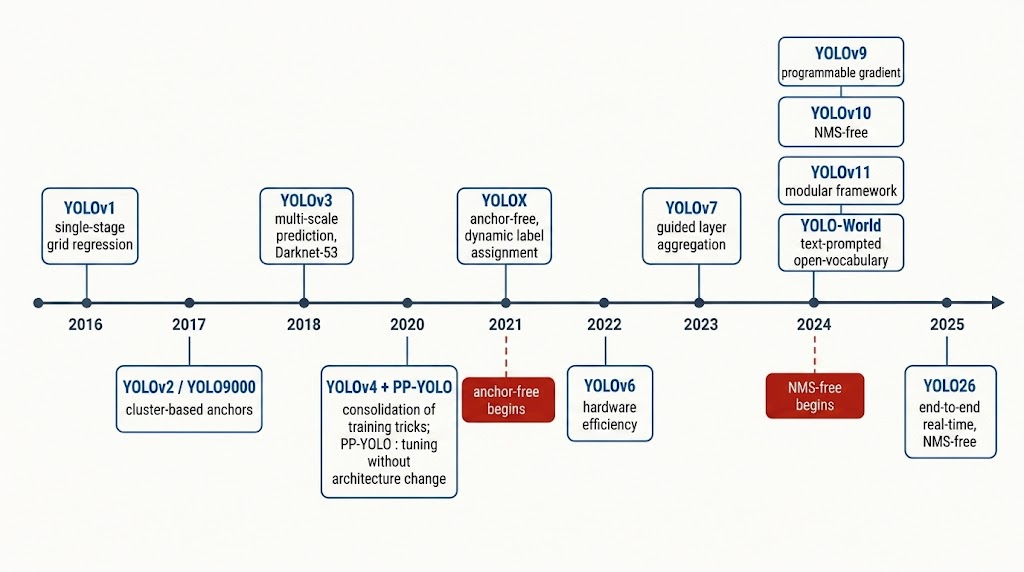
\includegraphics[width=\linewidth]{F02-timeline-yolo-gpt-image-2-en}
\caption{Supporting context for the YOLO family: design components used to address single-pass detection, including multi-scale prediction, decoupled heads, re-parameterization, and NMS-free inference.}
\label{fig:timeline}
\end{figure*}

YOLO removed the proposal stage by treating detection as one regression from the whole image to boxes and class probabilities. The image is divided into an $S\times S$ grid; each cell predicts a fixed number of boxes with confidence scores and one set of class probabilities, and a single network evaluation produces all detections \cite{redmon2016yolo}. The original model reached 63.4\% mAP on PASCAL VOC 2007 at 45 FPS, and the smaller Fast YOLO ran at 155 FPS. Because the network sees the whole image, it made fewer background errors than Fast R-CNN. The authors also stated the cost of the grid: each cell predicts only two boxes and one class, so small objects that appear in groups, their example being a flock of birds, are often missed, and the $7\times7$ grid limits how many objects one image can yield. A tree carrying ten bunches in a cluster behind a frond presents the same configuration.

The next two versions addressed that limitation directly. YOLOv2 replaced hand-chosen box shapes with anchor dimensions obtained by $k$-means clustering of the training boxes, constrained each box centre to its own grid cell to stabilize training, passed higher-resolution features forward through a passthrough layer, and trained on randomly varied input sizes, reaching 76.8--78.6\% mAP on VOC 2007 at 40--67 FPS \cite{redmon2017yolo9000}. Predictions were still made on one $13\times13$ grid, so small objects improved but were not solved. YOLOv3 added prediction at three scales in the manner of a feature pyramid, a residual Darknet-53 backbone, and independent logistic classifiers that allow overlapping labels, reaching 33.0\% AP (57.9\% AP50) on COCO at 51 ms per image \cite{redmon2018yolov3}. It became a common baseline in applied work, including the citrus detector discussed in Section~\ref{sec:identity}, although closely touching objects remained difficult and anchors still had to be tuned for each dataset.

Between 2020 and 2023 the family changed mostly in how it was trained and how its parts were arranged. YOLOv4 selected and combined training-time techniques (Mosaic augmentation, CIoU loss, self-adversarial training) with inexpensive architectural modules (CSP, SPP, PAN, Mish) and reached 43.5\% AP on COCO at about 65 FPS with a model that could be trained on one consumer GPU \cite{bochkovskiy2020yolov4}. YOLOX removed anchors, separated the classification and regression heads, and assigned training targets dynamically with SimOTA, reaching 50.0\% AP at 68.9 FPS in its large variant \cite{ge2021yolox}. YOLOv6 was designed for industrial deployment, with a re-parameterized EfficientRep backbone whose training-time branches merge into single convolutions at inference; its small variant reached 43.5\% AP at 495 FPS on a Tesla T4 \cite{li2022yolov6}. YOLOv7 pursued the same principle of accuracy gained at training time and removed at inference, with E-ELAN blocks, planned re-parameterization, and coarse-to-fine label assignment, and its E6E variant reached 56.8\% AP at 36 FPS on a V100 \cite{wang2023yolov7}. Gold-YOLO changed the neck instead: its Gather-and-Distribute mechanism collects features from all levels into one module and injects them back into each level, so information does not have to pass step by step through intermediate scales \cite{wang2023goldyolo}. For objects whose size depends on range, this is a change to the part of the network that decides which scale sees which object.

Much of this progress is difficult to attribute to architecture. One benchmark re-trained 33 models from seven YOLO versions on three datasets with uniform hyperparameters and hardware; the ranking changed with dataset and model size, with YOLO11 giving the most balanced accuracy and efficiency, YOLOv10 the highest efficiency, and YOLOv9 the highest accuracy on small data \cite{alif2024yoloevolution}. Together with PP-YOLO, which gained its accuracy from ten published training techniques added to an unchanged YOLOv3 \cite{long2020ppyolo}, this result implies that an FFB comparison must fix recipe, resolution, and hardware before it attributes a difference to the model.

The last three years turned attention to the final step of every earlier version: non-maximum suppression (NMS). All previous YOLO models were trained with one-to-many assignment, so one object produces several overlapping boxes, and NMS keeps the highest-scoring box and discards the others whose overlap exceeds a threshold. In a canopy this step decides counts. If two bunches overlap more than the threshold, one of them is discarded and two bunches become one detection; if the threshold is raised to keep them, a single bunch is more likely to survive as two boxes. YOLOv9 first addressed a different loss, the information that deep networks discard on the way to the output, by adding a reversible auxiliary branch (Programmable Gradient Information) that supplies reliable gradients during training and is removed at inference; YOLOv9-E reached 55.6\% AP on COCO \cite{wang2024yolov9}. YOLOv10 then removed NMS. It trains two heads on a shared body, one with one-to-many assignment for rich supervision and one with one-to-one assignment, and uses the same matching metric for both so that the object chosen by the second head is the best sample of the first. At inference only the one-to-one head remains. YOLOv10-S reached 46.3\% AP at 2.49 ms, 1.8 times faster than RT-DETR-R18 at similar accuracy \cite{wang2024yolov10}. YOLO11 added C3k2 blocks and the C2PSA spatial-attention module to the YOLOv8 design \cite{khanam2024yolov11}. YOLO26, the model used for the SawitMVC baseline, removes both NMS and the Distribution Focal Loss, adds a progressive loss and a small-target-aware label assignment (STAL), and reports 40.9--57.5\% mAP on COCO at 1.7--11.8 ms on a T4 across five model sizes \cite{sapkota2025yolo26}. YOLO-World added a separate capability, open-vocabulary detection, by coupling a YOLOv8 detector with CLIP text embeddings that are re-parameterized away at inference \cite{cheng2024yoloworld}; this matters when the class taxonomy of an inventory changes after the detector has been trained.

The YOLO literature does not yet include a model that removes the SawitMVC detection failure. YOLO26 is the newest generation examined here, and in the published baseline it reaches an AP50 of 0.354 on the least mature bunches \cite{indriani2026sawitmvc}. That baseline was deliberately untuned and trained at a 640-pixel input on $960\times1280$ images, so it is a reference point, not a ceiling. The reviews of the family relate its architecture, metrics, and applications \cite{jiang2022yoloreview,terven2023yolo,hussain2023yolo,vijayakumar2024yolo}, including its use in weed, crop, and disease detection \cite{sapkota2024yoloagri}, and a decadal review traces the recurring design choices across versions \cite{sapkota2025yologenesis}. None of them reports a controlled test of which component matters for occluded, range-varying fruit. A compact multi-scale YOLO is therefore a justified first RGB baseline when latency is constrained, and its selection should follow a field failure analysis of missed distant bunches, merged neighbours, and unstable identities, using the measurements in Table~\ref{tab:baseline}.

\subsection{Feature representation, attention, and query-based detection}

Backbone choice sets the balance of fine detail, context, and deployment cost. Residual shortcuts made deeply stacked convolutional features trainable \cite{he2016resnet}, and CBAM added inexpensive channel and spatial recalibration \cite{woo2018cbam}. The Vision Transformer made every feature globally contextual but needed large-scale pretraining \cite{dosovitskiy2021vit}; Swin and Swin V2 restricted attention to shifted local windows so that transformers could serve dense prediction at high resolution \cite{liu2021swin,liu2022swinv2}; and PVT built a progressively shrinking transformer pyramid \cite{wang2021pvt}. ConvNeXt is the necessary control for any claim about attention. It modernized a pure convolutional network with design choices taken from transformers, such as a patchify stem, $7\times7$ depthwise kernels, and fewer normalization layers, and matched or exceeded Swin; in Cascade Mask R-CNN on COCO, ConvNeXt-T reached 51.3 AP against 50.4 for Swin-T \cite{liu2022convnext}. A field comparison therefore has to separate a benefit of attention from a benefit of training recipe, resolution, or compute.

DETR approached instance formation from the opposite direction to NMS. It predicts a fixed set of boxes with a transformer encoder-decoder and trains them with bipartite Hungarian matching, so that each ground-truth object is assigned to exactly one prediction and duplicates are penalized by the loss itself \cite{carion2020detr}. With a ResNet-50 backbone it matched an optimized Faster R-CNN on COCO at 42.0 AP, performing better on large objects and worse on small ones, and it needed very long training. The following work repaired these two weaknesses one mechanism at a time. Deformable DETR replaced global attention with multi-scale deformable attention, in which each query samples a small number of learned points around a reference point on four feature levels; convergence became ten times faster and small-object accuracy rose, with the two-stage variant reaching 46.9 AP after 50 epochs \cite{zhu2021deformabledetr}. Conditional DETR separated content matching from spatial matching in cross-attention and reached 40.9 AP in 50 epochs, a 6.7-fold speed-up in convergence \cite{meng2021conditionaldetr}. DN-DETR traced part of the slow training to the instability of Hungarian matching in early epochs and added an auxiliary task of reconstructing noised ground-truth boxes, which bypasses the matching; it reached 48.6 AP in 50 epochs at no inference cost \cite{li2022dndetr}. DINO combined contrastive denoising, mixed query selection, and a look-forward-twice box update and reached 49.4 AP in 12 epochs with ResNet-50 \cite{zhang2023dino}. Co-DETR attached one-to-many auxiliary heads to the encoder during training only, enriching the supervision that one-to-one matching provides \cite{zong2023codetr}, which is the same remedy YOLOv10 later applied to a convolutional detector.

Real-time DETRs then competed with YOLO on its own terms. RT-DETR separated intra-scale from cross-scale feature interaction in a hybrid encoder and selected initial queries by minimum uncertainty, becoming the first transformer detector to run at real-time speed without NMS \cite{zhao2024rtdetr}. RF-DETR used weight-sharing neural architecture search on a DINOv2 backbone to derive a family of detectors from one training run, from 48.0 AP at 2.3 ms to 60.1 AP at 17.2 ms on COCO \cite{robinson2025rfdetr}. Le-DETR replaced the backbone and encoder with neighbourhood-attention components and reported 52.9--55.1 mAP at 4.45--6.68 ms on an RTX 4090 with about 80\% less pretraining data than RT-DETRv2 \cite{huang2026ledetr}. These models are appropriate comparators where contextual multi-scale reasoning is needed, but their data and deployment cost must be justified by a measured gain over a compact convolutional baseline on plantation data.

One-to-one assignment, whether in DETR or in YOLOv10 and YOLO26, gives each object one prediction inside one image. It says nothing about the next image. A bunch photographed from the north and from the east is two objects to every detector in this section, and the second detection is correct by every per-image metric. The SawitMVC baseline makes this concrete: an NMS-free detector feeding a naive sum would inherit the 1.89-fold duplication of the annotated boxes in addition to its own detection errors \cite{indriani2026sawitmvc}. The step that turns two correct detections into one inventory record lies outside the detector, and Section~\ref{sec:identity} examines it.

\begin{table*}[t]
\centering\small
\caption{Questions that turn detector comparison into FFB-relevant evidence.}
\label{tab:baseline}
\begin{tabular}{p{0.21\textwidth}p{0.32\textwidth}p{0.36\textwidth}}
\toprule
Question & Evidence to measure & Why it matters for FFB counting \\
\midrule
Can small and occluded bunches be found? & AP/recall by object size and occlusion stratum & Aggregate AP can conceal loss of distant or frond-covered bunches. \\
Does the detector separate instances? & Split/merge errors, instance recall, and per-tree count error & A box-level score does not expose a merged pair or a duplicate instance. \\
Can the system operate on the platform? & End-to-end latency, memory, power, and throughput on target hardware & FLOPs or desktop FPS are not field latency. \\
Does classification remain attached to the right bunch? & Per-instance maturity accuracy and calibration & Maturity labels are operational only when their associated bunch is correct. \\
\bottomrule
\end{tabular}
\end{table*}


\section{Evidence for cross-view identity and duplicate control}
\label{sec:identity}

A class-wise inventory needs an explicit rule for deciding whether two observations show the same physical fruit. The orchard literature has built such rules for a decade, and several studies measured where their rules failed. This section follows those studies in order, because each failure points to the part of the transferable literature that addresses it: camera pose and temporal association, monocular and sensor depth, three-dimensional localization, and confidence-aware geometric decisions.

\subsection{What the orchard studies measured about double counting}
\label{sec:orchard}

\paragraph{Statistical correction and its alternative.} The first answer to duplication was to calibrate it away. Koirala \textit{et al.}\ compared six detector architectures for mango and developed MangoYOLO, which reached an F1 of 0.968 and an AP of 0.983, yet converting its detections into an orchard load estimate still required a correction factor fitted against hand-harvest counts \cite{koirala2019deepfruit}. This is mechanism M1, and it has the strength that Stein \textit{et al.}\ measured: a single-view count calibrated in this way was the most repeatable estimate in their mango study \cite{ledger_r_408d13511cac4177}. Its weakness is that the factor describes an average tree. It cannot say which fruit was counted twice, and it has to be refitted whenever canopy geometry, cultivar, or acquisition changes. The SawitMVC divisor has the same form; it is computed from the training split and, on annotated boxes, leaves a mean bias of $+0.009$ bunches per class and tree \cite{indriani2026sawitmvc}.

\paragraph{Geometry as a correction step.} Liu \textit{et al.}\ (2018) kept a tracker but added geometry as a filter on its output. They segmented fruit with a fully convolutional network, linked detections between video frames with the Hungarian algorithm on costs from a Kalman-corrected KLT tracker, and then reconstructed the sequence with structure from motion (SfM), so that each track received a relative 3D position and size \cite{ledger_m_9966d81433d61ed3}. These estimates were used to reject outlier tracks and tracks that counted a fruit already counted. On oranges filmed in daylight with heavy occlusion and large depth variation, the uncorrected count had an L1 error of 593 fruit, a mean error of 17.1\%, and a standard deviation of 26.3\%; after the 3D correction the figures were 203, $-0.2\%$, and 7.8\%. On trellised apples filmed at night under controlled lighting, the correction mattered less, because the trellis kept fruit at similar distances and reduced occlusion. The geometry step therefore helped most under the conditions an oil-palm canopy presents. The authors listed one gap as future work: SfM from one camera gives only relative depth and size, and absolute scale would need an inertial sensor or a known fruit size.

\paragraph{Joining two sides of a tree.} Liu \textit{et al.}\ (2019) removed the expensive sensors and kept the geometry \cite{ledger_r_00f82e0f404d691b}. Their pipeline used a monocular camera only. It detected fruit and tree trunks with CNNs, tracked both with a Kalman filter that fused detector output with optical flow, and ran a semantic SfM that used the fruit and trunk tracks themselves as landmarks. This took about five minutes for a 1{,}000-frame video, against about ten hours for SIFT-based SfM. On a mango dataset its counts approached those of a reference system with a camera, LiDAR, and GPS/INS: the regression slope was 0.86 against 0.97, and $R^2$ was 0.78 against 0.88. The authors traced most of the remaining gap to trees with many fruit, and to one specific step. The two sides of each tree were recorded in separate passes and could not be reconstructed as one point cloud, so fruit landmarks from the two sides were separated by a rule based on the trunk centroid, and a landmark on the far side of the centroid was discarded as a presumed duplicate. Under heavy occlusion, a fruit beyond the centroid is often visible from one side only, and the authors identified this rule as a likely cause of the under-counting. This is the configuration of a four-position oil-palm census: separate photographs from opposite sides of one tree, with no continuous camera path joining them.

\paragraph{Detection and counting reward different methods.} H\"ani \textit{et al.}\ compared fruit detection and counting methods on the same apple datasets, which earlier studies had not done \cite{ledger_r_1358c0868a62c84a}. A semi-supervised Gaussian-mixture colour model had the highest detection F1 on six of seven datasets, while a CNN count regressor was more accurate for counting on all of them. The combination reached 95.56--97.83\% of harvested yield. The ranking of methods changed with the task, which supports evaluating detection and counting separately.

\paragraph{Tracking and the limit of appearance.} Video tracking (M3) was the next route. Zhang \textit{et al.}\ built OrangeYolo, a YOLOv3-derived detector with attention-based multi-scale fusion for small fruit that reached 0.957 mAP against 0.905--0.917 for YOLOv3, v4, and v5, and OrangeSort, which estimates fruit motion between frames and counts a fruit only when its track crosses a fixed counting region \cite{ledger_r_ee550a3e3a6fb318}. On six videos of 22 citrus trees the counting MAE was 0.081, against 0.45 for SORT and 1.212 for DeepSORT. DeepSORT, which adds a learned appearance descriptor to the motion model, was the worst of the three. Gené-Molá \textit{et al.}\ obtained the same ordering on apples \cite{ledger_r_2d972b94554c6cd1}. With a YOLOv5x detector, ByteTrack reached a HOTA of 0.6894, SORT 0.6804, and DeepSORT 0.6824, while DeepSORT took 128 ms per image against about 15 ms for the other two. The authors attributed the absence of a gain to the similarity of apples to one another, which leaves a re-identification network little to separate, and they noted that an earlier study had found the opposite. Their best counts reached a MAPE of 7.47\% one week before harvest. Hu \textit{et al.}\ reported that adding SORT-type tracking to an attention-augmented YOLOv7 reduced inter-frame counting MAE by 0.642 relative to the detector alone \cite{ledger_r_d594d85dc382f9ff}, and Abeyrathna \textit{et al.}\ tracked apples hung on artificial trees with DeepSORT from a vehicle at three forward speeds and three camera angles, using an RGB-D camera to place each counted apple for a robotic arm \cite{ledger_r_9e1316b934e66409}. Two separate studies thus found no benefit from appearance features for fruit that look alike. Neighbouring bunches of the same maturity class on one palm present a stronger version of that similarity.

\paragraph{What a total count hides.} Rapado-Rincón \textit{et al.}\ made the evaluation itself the subject \cite{ledger_r_700d34dae0f20d78}. Their robot carried an RGB-D camera on an arm around tomato plants and maintained a world model of fruit that was updated by multi-object tracking. The total count had a maximum error of 5.08\%, while the tracking accuracy, measured with HOTA, was at most 71.47\%. They argued that a correct total can hide identity switches, and false positives that cancel false negatives, so that count error alone cannot evaluate an association algorithm. The SawitMVC counters are evaluated by count error per class and tree \cite{indriani2026sawitmvc}; the dataset's identity links would allow the association itself to be scored as well.

\paragraph{Lifting the count into 3D.} Several studies moved the whole count into a 3D representation. Gené-Molá \textit{et al.}\ (2020) projected Mask R-CNN detections from many photographs of 11 Fuji apple trees into an SfM reconstruction and filtered the resulting 3D points with a support-vector classifier; against 1{,}455 hand-counted apples, F1 rose from 0.816 for 2D detection to 0.881, with precision increasing from 0.762 to 0.857 and recall from 0.878 to 0.906 \cite{genemola2020fruit3d}. Recall rose because a fruit partly hidden in one image was found in another and merged in 3D. FruitNeRF trained a semantic neural radiance field from posed monocular images and foundation-model fruit masks, sampled a fruit-only point cloud from it, and counted fruit by clustering that cloud, so that no tracking step was needed \cite{ledger_m_1210e3ea00486b68}. On synthetic trees it counted 283 of 283 apples but 926 of 1{,}150 mangoes and 651 of 781 plums, the fruit that grow closest together, and it needed 30 to 60 images per tree depending on resolution. Wang \textit{et al.}\ added semantic segmentation to ORB-SLAM3 on an autonomous vehicle to build labelled point-cloud maps of tomato plants \cite{ledger_r_b2e0e9aabad17a97}, and Park \textit{et al.}\ built 3D crop instances incrementally in real time and associated them by 3D generalized intersection-over-union \cite{park2026cropassociation}.

\paragraph{Where geometry fails.} Lee \textit{et al.}\ reported the most detailed failure analysis of a geometric count \cite{ledger_r_d4270ea8ab11f268}. A ground vehicle carried a LiDAR and a camera through a horizontal-trellis pear orchard, FAST-LIO2 built the 3D map and estimated the six-degree-of-freedom pose, and YOLOv11s detections were attached to map points and tracked over time. A new detection was merged with an existing fruit if the two lay within 0.075~m, a radius chosen to be smaller than the smallest pear diameter at harvest (83.2~mm) so that adjacent fruit would not be merged. On a $6\times70$~m plot the counting accuracy was 96.2\%, yet 53 fruit were still counted twice. Thirty duplicates lay inside the association radius and were missed by the temporal filter or the nearest-neighbour search; the other 23 arose where SLAM drift, 0.085~m in the example shown, exceeded the radius during the vehicle's turning manoeuvres. The radius could not be enlarged without merging neighbouring fruit. The same constraint applies to oil palm, where bunches on one palm grow in contact and the useful association radius is correspondingly small.

\paragraph{Learning the association.} The newest work learns the association function (M5). Fusaro \textit{et al.}\ segmented fruit instances in coloured point clouds from a terrestrial laser scanner and trained an attention-based network to match each fruit with its counterpart in a scan taken at an earlier session, including a probability that a fruit has no match \cite{ledger_r_0eda6374aaf85fae}. The method outperformed the compared baselines, but re-identification could be evaluated only on strawberries, because temporally consistent instance annotations did not exist for the other fruit, and segmentation errors propagated into the matching. The requirement for identity-annotated training data is the main cost of M5, and SawitMVC is one of the few fruit datasets that supply such annotations across views \cite{indriani2026sawitmvc}.

\paragraph{Consequences for a four-position oil-palm census.} Read together, these studies locate the failures that a cross-view mechanism for oil palm must survive. Appearance matching was not better than motion alone for look-alike fruit \cite{ledger_r_ee550a3e3a6fb318,ledger_r_2d972b94554c6cd1}. Tracking needs a continuous camera path, which four or eight separate photographs do not provide. Monocular geometry recovers relative position but not scale, and it lost fruit when two sides of a tree were joined by a coarse rule \cite{ledger_m_9966d81433d61ed3,ledger_r_00f82e0f404d691b}. Metric geometry removed most duplicates but not those caused by pose drift larger than the gap between neighbouring fruit \cite{ledger_r_d4270ea8ab11f268}, and 3D clustering under-counted the most tightly grouped fruit \cite{ledger_m_1210e3ea00486b68}. A correct total can conceal all of these errors \cite{ledger_r_700d34dae0f20d78}. The remaining subsections examine the transferable literature on each cause: camera pose under a moving canopy, depth and its scale, 3D localization, and confidence-aware geometric decisions.


\subsection{SLAM, camera pose, and temporal association (2017--2022)}

The pear study located the failure of a metric count in the pose estimate: during the vehicle's turns, SLAM drift exceeded the radius within which two observations were treated as one fruit \cite{ledger_r_d4270ea8ab11f268}. Camera pose is therefore part of the identity decision. A detector operates on one frame, while an inventory is defined over a traversal, and the connection between them is association: deciding whether an object in a new frame is an already-observed bunch or a new one, and this is the mechanism that converts good per-frame detection into a correct count. Appearance similarity alone is fragile in a plantation where neighbouring bunches look alike, and geometry alone is fragile where depth is incomplete or the camera pose is uncertain, so the count should emerge from the agreement of detection, instance separation, depth or projected position, camera motion, and temporal continuity. SLAM systems are the corpus's evidence on the camera-motion component, because they express successive views in a common coordinate frame. ORB-SLAM2 built a feature-based system on the fast, rotation-robust ORB descriptor that runs on monocular, stereo, and RGB-D cameras with tracking, local mapping, and loop closure, differing across sensors only in how each feature's depth is obtained \cite{murartal2017orbslam2}. ORB-SLAM3 extended this to a unified visual, visual-inertial, and multi-map system, formulating visual-inertial initialization as a maximum-a-posteriori estimation from the start and supporting pinhole and fisheye models \cite{campos2021orbslam3}. DROID-SLAM took the learned route, embedding a differentiable dense bundle-adjustment layer inside a recurrent network that iteratively updates optical flow and pose across monocular, stereo, and RGB-D input \cite{teed2021droidslam}. These provide the common frame in which two detections can be tested for spatial compatibility, but a plantation violates the static-world assumption most SLAM systems make.

The dynamic-scene branch applies to plantations because moving fronds and self-similar texture corrupt pose estimation. DynaSLAM extends ORB-SLAM2 with two complementary signals, a Mask R-CNN semantic prior that flags a-priori movable classes and multi-view geometric verification that detects actual motion, and discards features on dynamic regions before they are used for pose or mapping \cite{bescos2018dynaslam}. DS-SLAM runs semantic segmentation (SegNet) and epipolar motion-consistency checking as two parallel processes and combines them to decide which objects are truly moving, cutting trajectory error sharply in dynamic scenes \cite{yu2018dsslam}. CFP-SLAM replaces the binary static/dynamic label with a continuous probability computed coarse-to-fine, from the object level (a YOLOv5 detection) down to individual keypoints, using optical-flow and epipolar constraints \cite{hu2022cfpslam}, a graded-confidence approach that mirrors the quality-gating seen in the depth and fusion literature. Soares \textit{et al.}\ contribute the methodological template most useful to this review: they inserted YOLO and Mask R-CNN, in turn, at an identical dynamic-object-filtering position in ORB-SLAM2 while holding every other component fixed, isolating the accuracy-versus-speed trade-off of the detector choice as a single controlled variable \cite{soares2019visualslam}. An FFB study that asks whether a heavier detector earns its cost needs the same control. None of these systems counts objects, but together they show how camera pose and dynamic-content handling make cross-frame association geometric rather than a naive appearance match, and that the reliability of that association in vegetation is an empirical question, not a free assumption.

There are at least four counting failure modes to report separately: a bunch missed in every frame, two nearby bunches merged into one instance, one bunch split into several, and a bunch correctly detected repeatedly but never linked: a duplicate count. Image-level AP responds mostly to the first three; absolute count error per tree, per row, or per traversal is needed to expose the fourth. A geometry-aware association policy can be expressed as a sequence of gates: check detector confidence and maturity label; check whether the depth observation is valid and compatible with the candidate instance; project the candidate into a common frame using the current pose estimate and compare it to the uncertainty region of existing records; and finally resolve competing matches by appearance and temporal continuity. When the depth or pose gate fails, the system should fall back to RGB tracking as a weaker cue and report the degraded condition rather than treating unavailable geometry as a zero measurement. This yields clean ablations: appearance-only association, depth without pose, pose-aware geometric association, and a quality-gated variant, each reporting count error alongside false merges, false new records, and unresolved observations.



\subsection{Monocular depth (2014--2026)}

The monocular orchard pipelines placed fruit relative to one another but not in metres, and their authors named absolute depth and size as the missing quantity \cite{ledger_m_9966d81433d61ed3}. Depth can be supplied by a registered RGB-D sensor, by stereo reconstruction, or by a depth-prediction model operating on RGB alone. These sources must not be collapsed into one variable, and the monocular-depth literature is the clearest record of how the field learned what a predicted depth map does and does not mean. Two surveys anchor the arc: Ming \textit{et al.}\ organized 2014--2020 methods by supervision signal, because that choice determines the dataset, the loss, and whether the output is metric or merely relative \cite{ming2021depthsurvey}; and a more recent survey traces monocular \emph{metric} depth from geometry-based methods to current foundation models, the distinction that matters when an FFB task reports a physical range \cite{zhang2025metricdepthsurvey}.

The supervised branch began with Eigen \textit{et al.}, who were the first to predict a dense depth map from a single RGB image with a deep network and who already identified the problem that shapes the entire field: absolute per-pixel depth from one image is ill-posed, so the network is trained on a scale-invariant error that measures depth \emph{relations} (which pixel is nearer, by what ratio) rather than absolute values. A coarse network reads the whole image to capture global layout, and a fine network refines it locally \cite{eigen2014depth}. This scale-invariance is the reason a monocular depth map cannot be treated as a distance measurement without extra calibration, a caveat that propagates directly to any FFB pipeline that would use predicted depth to place a bunch in space. BTS inherited the supervised setting and improved how coarse features become fine depth: instead of blindly upsampling, each feature cell at reduced resolution predicts the four coefficients of a local 3D plane, and depth for every pixel in the corresponding patch is computed from that plane, injecting a geometric prior into the decoder \cite{lee2019bts}. AdaBins reconsidered the output representation itself, arguing that a fixed discretization of the depth range is wasteful: a transformer module reads the whole scene and predicts per-image adaptive bin widths, and the final depth is a bin-centre expectation, so the model spends resolution where the particular image needs it \cite{bhat2021adabins}. DPT then swapped the convolutional encoder for a Vision Transformer and exploited the property that token count never changes through the layers, assembling tokens from several depths into multi-resolution feature maps that give dense prediction a constantly global receptive field \cite{ranftl2021dpt}. NeWCRFs kept the accuracy-through-structure idea but expressed it as optimization, computing a fully-connected conditional random field within each local window via multi-head attention over a Swin backbone, so neighbouring depth predictions are made mutually consistent at tractable cost \cite{yuan2022newcrfs}. Across this branch the trajectory is from raw regression toward ever-stronger geometric and structural priors, but all of it still requires dense ground-truth depth for training, the constraint the next branch removes.

A parallel self-supervised branch removed the need for depth labels by turning depth into a by-product of image reconstruction, attractive for agriculture, where dense ground-truth depth is expensive or impossible to collect in the field. Godard \textit{et al.}\ reasoned that a function able to synthesize the right-hand stereo view from the left must implicitly encode scene geometry; that geometry is expressed as a disparity map, and a left-right consistency constraint enforces that the two predicted disparities agree, so the network learns depth from stereo pairs alone with no depth labels \cite{godard2017monodepth}. Monodepth2 inherited this setup and, rather than enlarging the model, fixed how the reconstruction error is computed: it takes the per-pixel \emph{minimum} reprojection error over multiple source frames (so an object occluded in one frame is not penalized), auto-masks pixels that do not move relative to the camera (removing a common failure on scenes with a moving-with-camera object), and samples the loss at multiple scales \cite{godard2019monodepth2}. These loss-level corrections, not architecture, produced the gains, a reminder that in self-supervised depth the supervision signal is the design surface. PackNet attacked the detail-loss problem of downsampling by replacing lossy pooling with a symmetric 3D packing/unpacking operation that moves spatial detail into the channel dimension and back, learned with 3D convolutions, and trained self-supervised from monocular video \cite{guizilini2020packnet}. MonoIndoor adapted the paradigm to the indoor setting, whose depth range varies wildly between rooms, by factorizing the prediction into a single global scale (one number for the whole image) and a scale-free relative depth map, with the global scale predicted separately \cite{ji2021monoindoor}. That scale/shape factorization is important beyond indoors: it reappears as the organizing idea of the metric-depth foundation models below, and it is the decomposition an FFB system needs if it wants scene structure from cheap monocular depth while treating absolute scale as a separately-calibrated quantity.

The recent shift is toward zero-shot, cross-dataset robustness and, eventually, metric transfer, the property that would let a depth model trained elsewhere be used on a plantation without retraining. MiDaS made the enabling observation that many applications need not absolute metric depth but correct relative structure (which is nearer, by how much); if the training target is only relative depth, then datasets with incompatible scales and offsets can be mixed, so MiDaS trained on five heterogeneous datasets with a scale-and-shift-invariant loss in disparity space and generalized far better across scenes than any single-dataset model \cite{ranftl2022midas}. Metric3D then confronted the reason relative models cannot report metres: the same object at the same distance produces a different pixel size under different focal lengths, so scale is fundamentally ambiguous across cameras. Rather than let the network guess the camera, Metric3D transforms every image into a canonical-camera space with a simple geometric operation before the network sees it, removing focal-length ambiguity and enabling zero-shot \emph{metric} prediction when the intrinsics are known \cite{yin2023metric3d}. ZoeDepth reached metric depth by a two-stage route that revives the MonoIndoor factorization at scale: relative-depth pretraining on twelve datasets learns robust structure, and lightweight metric bins with attractor layers, fine-tuned per domain, attach an absolute scale \cite{bhat2023zoedepth}.

The foundation-model era moved the bottleneck from labels to images. Depth Anything scaled supervision from $\sim$1.5M labelled images to roughly 62M automatically pseudo-labelled unlabelled images, using a teacher model to annotate the cheap and diverse unlabelled data, and became a robust general-purpose relative-depth backbone \cite{yang2024depthanything}. Depth Anything V2 separated the two things the previous model conflated, label accuracy and data diversity, by training a very large ViT-Giant/DINOv2 teacher on 595K precisely-labelled \emph{synthetic} images and using it to pseudo-label a large real corpus, sharpening detail while keeping generalization \cite{yang2024depthanythingv2}. Marigold took an orthogonal route, repurposing the latent U-Net of a pretrained Stable Diffusion image generator into an affine-invariant depth estimator by casting depth as a conditional denoising problem, trained only on synthetic data yet transferring well to real images \cite{ke2024marigold}, evidence that a strong visual prior can substitute for large labelled depth corpora. The current frontier pushes on views, cameras, latency, and controllability, and each axis matters for a field system. Depth Anything 3 shows that a single plain transformer with a depth-ray prediction target can recover geometry consistent across arbitrary views, merely by re-arranging tokens across views \cite{lin2025depthanything3}. UniDAC generalizes metric depth to perspective, fisheye, and other camera models by predicting a scale-free shape branch and a separate scale branch and combining them \cite{ganesan2026unidac}, again the shape/scale split, now made camera-universal. AsyncMDE targets the latency wall a foundation model creates on a moving platform, amortizing a frozen Depth Anything V2 ViT-B (97.5M parameters) through a 3.83M-parameter fast asynchronous path so depth can be produced in real time \cite{ma2026asyncmde}. FocusDepth couples a segmentation prompt (SAM) with a depth foundation model through a fusion module so prediction can be focused on a chosen region \cite{du2026focusabledepth}, conceptually the ability to say ``give me depth for this bunch,'' which is what an instance-constrained depth sample requires. None of these advances, however, converts a predicted relative map into a valid distance measurement by itself, and the correlated-error problem is acute for FFB use: a pseudo-depth map derived from RGB shares its errors with the very image that generated it, so it is a structural prior rather than an independent sensor observation. Any FFB task that reports physical range, bunch position, or inter-frame geometric association must therefore declare which kind of depth it uses, calibrate and evaluate that interpretation explicitly, and down-weight depth wherever it contains holes, boundary artefacts, or a confidence failure under direct sunlight.



\subsection{Three-dimensional perception (2017--2023)}

A depth value becomes useful for identity only after it has been converted into a position that can be compared between views. RGB-D detection is not the same as three-dimensional perception. A box contains foreground, background, and often a mixture of depth layers, so a proposed FFB pipeline should not treat an arbitrary centre-pixel depth as a bunch range; it should use robust statistics over a valid instance region and retain an uncertainty value. The autonomous-driving 3D-detection literature is the richest record of how the field learned to turn depth and geometry into reliable object localization, surveyed by Arnold \textit{et al.}\ along the axis of sensor modality and data representation \cite{arnold2019survey3d}.

The lineage begins with the problem of how to represent an unordered point cloud so a network can process it, and each answer trades accuracy against speed. MV3D projected LiDAR into two structured 2D views, bird's-eye (BEV) and front view, so ordinary convolutions apply, and used BEV as the main proposal source because a top-down view preserves physical object size; it fused these with RGB through region-based deep fusion \cite{chen2017mv3d}. AVOD inherited this framework and moved the BEV-RGB fusion as early as possible, into the region-proposal network itself, so proposals consider both modalities from the start rather than validating them late, using a high-resolution FPN-style extractor \cite{ku2018avod}. VoxelNet removed the hand-designed projection by discretizing space into voxels and learning voxel features end-to-end from raw points with a Voxel Feature Encoding layer \cite{zhou2018voxelnet}, but 3D convolution over voxels is slow; PointPillars fixed this by collapsing the height axis into vertical ``pillars'' so the entire detector runs in efficient 2D convolutions, fast enough for real-time \cite{lang2019pointpillars}. PointRCNN inverted the usual order, first segmenting foreground points and letting each such point propose a box bottom-up rather than guessing box locations from anchors \cite{shi2019pointrcnn}, and PV-RCNN combined the two representations, using efficient sparse-voxel convolution to generate proposals and point-based set abstraction at a small number of keypoints to enrich them before refinement \cite{shi2020pvrcnn}. Frustum PointNets is the member of this family closest to an FFB pipeline because it states most clearly the ``detect in 2D, localize in 3D'' decomposition a bunch-counting pipeline would use: a 2D detection box on the RGB image is projected into a 3D viewing frustum, and a sequence of PointNets then segments and regresses the object only within that narrowed region \cite{qi2018frustum}. The pseudo-LiDAR line carries an equally important lesson about representation: Wang \textit{et al.}\ showed experimentally that the same depth data yields far better 3D detection when stored as a back-projected point cloud than as a front-view depth map, because 3D convolutions then operate in a physically meaningful space \cite{wang2019pseudolidar}, and Pseudo-LiDAR++ improved the source depth by retraining the stereo network directly on depth error rather than disparity error \cite{you2020pseudolidarpp}. For an FFB system these two results caution that how a depth measurement is represented can matter as much as its raw accuracy.

Camera-LiDAR fusion then matured toward learned, calibrated association. PointPainting decorates each LiDAR point with the semantic-segmentation class scores of the image pixel it projects to, before any 3D detector runs, a simple sequential fusion that lifts several detectors at once \cite{vora2020pointpainting}, and 3D-CVF aligns camera features into the LiDAR BEV space through an auto-calibrated projection and fuses them with location-dependent adaptive gating rather than uniform weights \cite{yoo20203dcvf}. CenterPoint reframed 3D detection, like its 2D cousin CenterNet, as centre-point heatmap prediction on BEV and thereby simplified multi-object tracking to centre association across frames \cite{yin2021centerpoint}, which corresponds to the counting problem, where tracking centres across a traversal is the association task. The transformer wave replaced fixed point-to-pixel correspondence with learned soft association: TransFusion represents each candidate as an object query that attends over both LiDAR and image features in two decoder layers, robust to calibration error \cite{bai2022transfusion}; BEVFormer builds a learnable BEV query grid filled by spatial attention over current-frame cameras and temporal attention over the previous BEV, adding a time dimension \cite{li2022bevformer}; DETR3D lets each learned 3D object query project its own reference point into every camera to gather features, so the query decides which view is relevant \cite{wang2022detr3d}; and BEVFusion encodes each modality independently into a shared BEV space before fusing, so neither is projected onto the other and each survives the other's failure \cite{liu2023bevfusion}. None of these is an FFB solution: they use LiDAR, driving-scale scenes, and calibrated multi-camera rigs absent from a plantation. As a body, though, they establish the coordinate-frame discipline a counting pipeline needs. What geometry adds is the ability to distinguish look-alike regions, to reject a re-observation at a previously mapped location, and to estimate reachability, and every one of these requires explicit intrinsics, registration, and depth-scale handling rather than an unqualified centre-pixel depth read from a box.

\subsection{Object pose and robotic grasping (2015--2024)}

Pose estimation and grasping are transferable as method evidence because both must reason about instance boundaries, geometry, occlusion, and coordinate transforms before a robot acts, and both make the confidence of that reasoning explicit, which is the analogue of deciding whether to commit a new inventory record. Hoque \textit{et al.}\ survey the shared taxonomy of 3D detection and 6D pose across RGB, depth, and RGB-D inputs \cite{hoque2021posesurvey}.

For 6D pose the guiding idea, established by PoseCNN, is to decompose the task by the visual nature of each parameter: translation determines where an object appears and how large it looks, rotation determines its surface appearance, so translation is recovered geometrically from per-pixel centre-direction voting plus a depth estimate while rotation is regressed separately, all in cluttered scenes \cite{xiang2018posecnn}. DenseFusion inherited the RGB-D setting and replaced global fusion with dense local fusion: the depth map becomes a point cloud via the camera intrinsics, each point is paired with its aligned colour feature, one pose is predicted per point, and a learned selection step picks the most reliable, an architecture built around the fact that some points are more trustworthy than others \cite{wang2019densefusion}. PVN3D moved keypoint detection out of the image plane into 3D, training each point to vote an offset toward each target 3D keypoint and solving for pose by least squares, which is more robust to occlusion than 2D keypoints \cite{he2020pvn3d}, and G2L-Net decomposed the problem into a global-to-local sequence: global localization by a 3D sphere, then translation and rotation in the object's own frame, to run in real time \cite{chen2020g2lnet}. FFB6D, whose acronym coincides with fresh-fruit-bunch work but denotes ``full flow bidirectional,'' exchanges RGB and geometry features in both directions at every encoder and decoder layer, so each branch is continuously informed by the other rather than fused once at the end \cite{he2021ffb6d}, the most thorough expression of the bidirectional-fusion principle seen throughout the RGB-D literature. The remaining methods broaden applicability: GDR-Net unifies dense 2D-3D correspondence with end-to-end differentiable direct regression \cite{wang2021gdrnet}; ZebraPose encodes an object's surface as a hierarchical binary code predicted densely per pixel, turning continuous coordinate regression into coarse-to-fine classification \cite{su2022zebrapose}; OnePose reframes pose as visual localization against a structure-from-motion model built from a reference video, needing no CAD model or per-object training \cite{sun2022onepose}; and FoundationPose unifies estimation and tracking of \emph{novel} objects through render-and-compare over a neural implicit representation, a foundation-model approach that removes the per-object assumption entirely \cite{wen2024foundationpose}. The transferable pattern for FFBs is the confidence-aware decomposition these methods share: constrain the geometry to a hypothesized instance, estimate a meaningful state, and quantify how reliable that estimate is.

Grasping supplies the closest analogue in the corpus to committing an action under geometric uncertainty: the decision to add one inventory record, update an existing one, or defer. Lenz \textit{et al.}\ framed grasp detection as binary classification over oriented candidate boxes from RGB-D, the direct transfer of object-detection thinking to manipulation \cite{lenz2015grasp}, and GG-CNN reframed it as per-pixel regression, predicting a grasp quality, angle, and width at every pixel of a depth image in a single tiny 62{,}420-parameter forward pass fast enough to close the control loop \cite{morrison2018ggcnn}. GR-ConvNet kept the per-pixel formulation but strengthened it with a generative residual architecture predicting quality, angle, and width maps from RGB-D \cite{kumra2020grconvnet}, and GR-ConvNet v2 refined the same design with Mish activation, dropout, and the Ranger optimizer to reach roughly 98\% grasp accuracy \cite{kumra2022grconvnetv2}. The 6-DoF branch moved from planar grasps into full clutter: VGN turns grasp detection into dense regression over a truncated signed-distance volume, emitting a quality, orientation, and width per voxel \cite{breyer2021vgn}, and Contact-GraspNet shrinks the search space by anchoring each grasp to an observed point on the object surface, so three of the translation degrees of freedom are fixed by the data \cite{sundermeyer2021contactgraspnet}. BCMFNet adds bilateral cross-modal attention so RGB and depth query each other before fusion, the grasping instance of the bidirectional-fusion idea \cite{zhang2023bcmfnet}. Two datasets underwrote this progress by replacing human labelling with computation: Jacquard generated grasp labels entirely through physics simulation on ShapeNetSem CAD models, yielding over 54k rendered images of 11k objects with more than one million successful grasp annotations \cite{depierre2018jacquard}, and GraspNet-1Billion analytically scored over 1.1 billion grasps across 190 scenes and 97{,}280 RGB-D images from two cameras \cite{fang2020graspnet}, a scale worth noting for an FFB program, since a similar analytic or simulated labelling strategy could reduce the annotation burden of a plantation dataset. The transferable decomposition for counting is thus: identify an instance, estimate a geometrically meaningful state, assess confidence, and commit only when the state is adequate, a conservative policy preferable to adding every high-score box to the total.



\subsection{Comparative implications of M0--M5}

The six mechanisms should be compared by the information they require before comparing their reported accuracy. M0 is a within-image count and is appropriate only when acquisition guarantees that an instance cannot reappear. M1 applies a calibrated correction to image-level counts; it can be useful for a stable, repeated acquisition protocol, but it cannot identify which particular bunch was duplicated. M2 uses appearance re-identification, so it is attractive when camera pose and depth are unavailable, yet its core assumption is weak in a canopy: adjacent bunches can share colour, texture, scale, and partial occlusion. M3 makes identity a temporal state, which requires sufficient frame-rate, bounded object displacement, and reliable handling of entry and exit from the field of view. M4 tests correspondence in a common geometric frame and can therefore reject a visually similar but spatially distinct bunch, but it requires calibrated intrinsics, an interpretable depth source or reconstruction, and a pose estimate whose uncertainty is carried into the match. M5 learns multi-view correspondence directly and may absorb appearance and geometry jointly, but it introduces a domain-specific training, annotation, and validation burden. Thus no mechanism is ``duplicate control'' in the abstract: it is a claim about what observations are available and which error source is being controlled.

This comparison also distinguishes two levels of validation. At the association level, a study should report pairwise match precision and recall, ID switches, false merges, false new records, and unresolved observations. At the inventory level, it should report absolute and relative count error by tree, row, or traversal, class-wise count error, and the proportion of records committed under degraded sensing. Per-image AP, even stratified by object size and occlusion, evaluates instance formation but cannot reveal whether one correctly detected bunch was entered into the inventory twice. Conversely, an apparently good total count can mask compensating errors in which one bunch is merged and another is duplicated. The M0--M5 comparison therefore needs an error decomposition: missed instances, split instances, merged instances, duplicate records, and unassigned records. Table~\ref{tab:metrics} makes this distinction operational.

The strongest field design is not necessarily the most complex mechanism. A short, non-overlapping traverse with a fixed camera pose may justify M0 or M1, whereas an informal walk-around sequence requires M3 or M4 before a total can be treated as an inventory. M2 is a sensible fallback when geometry fails, but should be labelled as such and not silently substituted for a pose-aware match. M4 is the most interpretable route when registered depth and camera motion are reliable; its confidence gate can withhold a record when depth holes, calibration drift, dynamic foliage, or poor localization make the match indeterminate. M5 becomes defensible when repeated viewpoints and annotated identities are sufficiently abundant to demonstrate generalization across trees, illumination, cultivars, and class attributes. These distinctions explain why agricultural studies with similar detection scores can reach very different counting reliability, and why a direct FFB benchmark must specify its acquisition protocol before it can claim a best association method.



\section{Multimodal geometry, agricultural evidence, and research priorities}
\label{sec:multimodal}

The orchard studies used depth and geometry to decide whether two observations were one fruit. The second failure in the SawitMVC baseline is different: the detector misses or misplaces bunches before any association starts, and the least mature class is found least often \cite{indriani2026sawitmvc}. This section asks whether a second modality can reduce that failure, what the fusion literature says about where and when depth should enter a network, and what the direct oil-palm evidence supports.

\subsection{RGB-D fusion for dense prediction}
\label{sec:fusion}

\begin{figure*}[t]
\centering
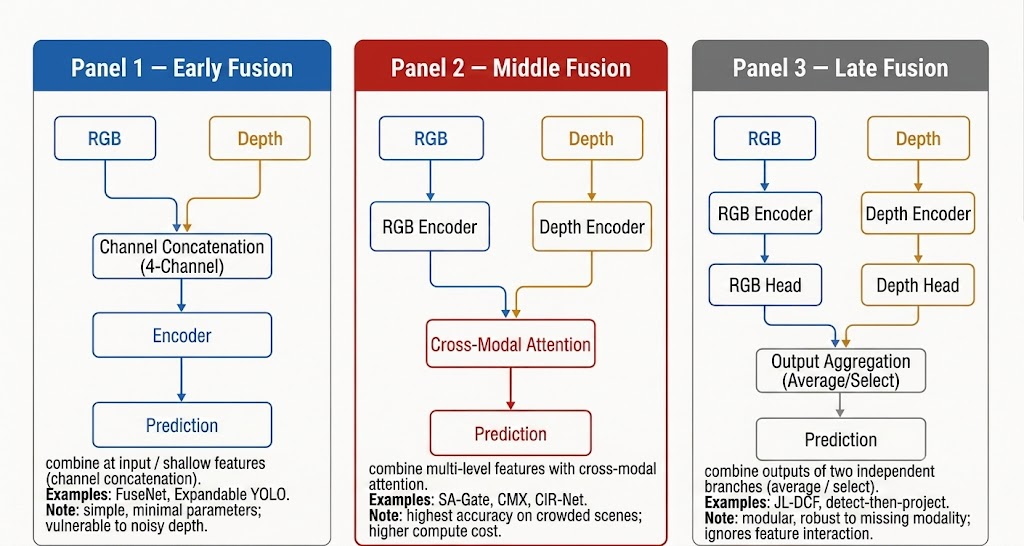
\includegraphics[width=\linewidth]{F04-strategi-fusi-gpt-image-2-en}
\caption{The three fusion locations that structure the RGB-D literature. Early fusion concatenates colour and depth at the input (for example FuseNet, Expandable YOLO); middle/feature fusion learns modality-specific representations before exchanging them at selected scales; late fusion combines predictions and supports an explicit RGB fallback.}
\label{fig:strategi}
\end{figure*}

The fusion literature asks two questions about depth: \emph{where} in the network the modalities should be combined, and \emph{how} the network should behave when depth is unreliable. Early fusion concatenates RGB and depth at the input; feature (middle) fusion learns modality-specific representations before exchanging them; late fusion combines predictions (Figure~\ref{fig:strategi}). These are competing experimental conditions, not cosmetic variants, and three sub-literatures in the corpus, RGB-D salient-object detection, RGB-D semantic segmentation, and RGB-D detection, each explored them in depth.

\subsubsection{RGB-D salient-object detection (2019--2025)}

Salient-object detection (SOD) is the sub-literature that confronted depth quality most directly, and it is therefore the most instructive for an FFB system that cannot assume clean depth; the space is surveyed by Zhou \textit{et al.}, whose taxonomy classifies methods by how and where depth is fused \cite{zhou2021rgbdsurvey}. The early methods each proposed a different answer to ``how should a depth map enter the network,'' and reading them in sequence exposes the design space. DMRANet refused to add raw depth to RGB, instead transforming depth at each level into a residual complement so that RGB remains the backbone and depth only supplies the missing cue, combined through multi-scale recurrent attention \cite{piao2019dmra}. BBS-Net treated multi-level features differently by their character rather than fusing them all at once: high-level ``teacher'' features first produce a coarse saliency map that gates the low-level ``student'' features, with a separate depth-enhancement module \cite{fan2020bbsnet}. JL-DCF took the opposite, minimalist stance: treat the depth map as just another image and push both modalities through one shared siamese backbone, so a single set of weights learns to serve both \cite{fu2020jldcf}. S2MA fused not the features but the modalities' non-local attention affinities, adding each modality's self-affinity matrix to the other's so geometry-based and appearance-based notions of ``which positions relate'' reinforce each other \cite{liu2020s2ma}. HDFNet reframed depth's role entirely, using it not as a fused feature but as the generator of input-specific dynamic convolution kernels, so depth decides \emph{how} RGB is filtered \cite{pang2020hdfnet}. UC-Net was the first to model the uncertainty of human annotation itself with a conditional variational autoencoder, predicting a distribution of plausible saliency maps rather than one deterministic answer \cite{zhang2020ucnet}, and CoNet made a choice with direct deployment value: it uses depth only as a training-time collaborative signal (alongside edge and saliency heads sharing an RGB encoder), so that at inference no depth map is required at all \cite{ji2020conet}. For a plantation where depth may be intermittently unavailable, a model that needs depth only during training is an attractive template.

D3Net treats depth as an optional input that must pass a quality test before it is trusted. It produces three saliency maps (from RGB alone, from the fused pair, and from depth alone), and a gating mechanism down-weights a low-quality depth map, the behaviour an outdoor FFB system needs when active depth fails under sunlight \cite{fan2020d3net}. The transformer wave then rebuilt SOD on attention. VST posed saliency as sequence-to-sequence prediction over patch tokens in one framework unifying RGB and RGB-D, so long-range dependencies across the image are modelled at every layer \cite{liu2021vst}, and TriTransNet strengthened the top three feature levels with three weight-shared transformer encoders where attention is affordable, refining depth features alongside \cite{liu2021tritransnet}. A cluster of methods refined how depth informs RGB: DSA2F splits the raw depth map into regions by its histogram modes and turns each into a spatial attention mask over RGB \cite{sun2021dsa2f}; DCF makes the quality problem explicit by first calibrating raw depth against the RGB image and only then fusing, separating correction from combination \cite{ji2021dcf}; and SPNet preserves RGB-specific, depth-specific, and shared streams in parallel so specificity is not lost in a premature merge \cite{zhou2021spnet}. The most recent methods combine strong backbones with bidirectional fusion: SwinNet drives edge-aware RGB-D and RGB-T SOD with dual Swin backbones and spatial-then-channel cross-modal alignment \cite{liu2021swinnet}, CIR-Net interacts the modalities at both encoder and decoder through a three-stream design \cite{cong2022cirnet}, and MobileSal shows the efficiency ceiling by restoring depth information only during training and reaching 450 FPS at deployment \cite{wu2022mobilesal}, a data point that a quality-aware depth branch need not be expensive at inference. HiDAnet exploits hierarchical depth granularity, discretizing the depth histogram with multi-Otsu into regions that align with the network's own coarse-to-fine hierarchy \cite{wu2023hidanet}; CAVER unifies RGB-D and RGB-T through a view-mixed transformer that treats fusion as a sequence of context updates by shared attention units \cite{pang2023caver}; and GL-DMNet replaces one-way fusion with parallel position-mutual and channel-mutual modules so RGB and depth filter each other bidirectionally \cite{yi2025gldmnet}. Across a decade of SOD work, the transferable result is that fusion should enable cross-modal correction and reduce dependence on an unreliable depth observation, but every one of these results is on saliency benchmarks with clean indoor depth, not on agricultural boxes under field conditions, so they justify testing quality-aware fusion for FFBs rather than asserting it will help.

\subsubsection{RGB-D semantic segmentation (2016--2025)}

\begin{figure}[t]
\centering
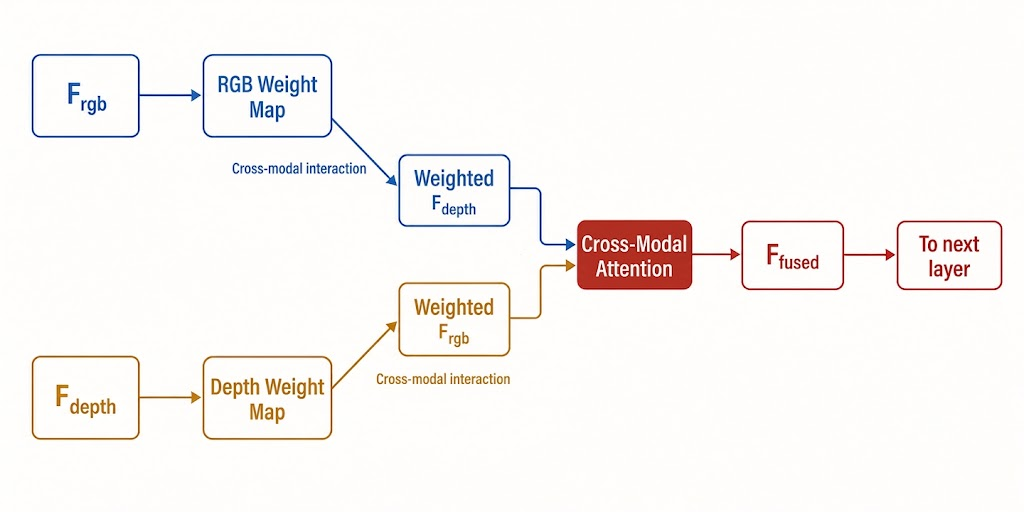
\includegraphics[width=\linewidth]{F06-atensi-lintasmodal-gpt-image-2-en}
\caption{The cross-modal attention mechanism that recurs across the strongest RGB-D methods (for example SA-Gate, CIR-Net, CMX): each modality generates a weighting map that gates the other before fusion, so a faulty depth measurement can be suppressed rather than allowed to contaminate the joint representation.}
\label{fig:atensi}
\end{figure}

Semantic segmentation traced the same fusion-location question but under dense per-pixel supervision, which makes its architectural conclusions unusually clean. FuseNet set the template that most later work varies: give depth its own encoder branch identical to the RGB branch and combine the two at the feature level rather than at the pixel level, summing depth features into the RGB branch at several stages \cite{hazirbas2016fusenet}. RDFNet inherited the two-branch idea and made the fusion learnable and residual, extending RefineNet so colour and HHA-encoded depth are fused through trained residual blocks at four resolutions before multi-resolution refinement \cite{park2017rdfnet}. RedNet showed that a deep RGB-D encoder-decoder trains well if every unit is residual and supervision is applied not only at the output but at intermediate layers \cite{jiang2018rednet}. ACNet separated two questions that earlier work had conflated, how the architecture preserves each modality's feature flow and how the network decides each modality's contribution per location, answering the first with three parallel branches and the second with channel-attention modules that weight RGB against depth pixel by pixel \cite{hu2019acnet}. SA-Gate applied the same idea to segmentation by filtering each modality before fusion. A cross-modal gate, computed from the other modality, suppresses features arising from a faulty depth measurement before they can contaminate the joint representation \cite{chen2020sagate}, the segmentation counterpart of D3Net's quality gate and a strong candidate mechanism for FFB depth that fails intermittently. This bidirectional cross-modal gating, shared by the strongest RGB-D methods, is illustrated in Figure~\ref{fig:atensi}.

The efficiency and transformer branches followed. ESANet demonstrated that two efficient shallow encoders (factored ResNet-34 blocks) with cheap Squeeze-and-Excitation depth fusion can rival much heavier RGB-D methods at deployment-friendly latency, a direct relevance for on-platform inference \cite{seichter2021esanet}, and ShapeConv made convolution itself depth-aware by decomposing each depth patch into a base component (its mean, that is, where it sits relative to the camera) and a shape component (the residual local relief), processing them separately \cite{cao2021shapeconv}. SegFormer contributed a simple, strong RGB backbone-decoder design: a hierarchical MiT encoder without explicit positional encoding plus a lightweight MLP decoder, which many RGB-D methods adopt as their base \cite{xie2021segformer}. TokenFusion addressed multimodal transformers economically by detecting uninformative token slots via a learned score and reusing them for tokens from the paired modality rather than adding tokens \cite{wang2022tokenfusion}. EMSANet solved semantic, instance, and panoptic segmentation plus orientation and scene classification from one shared RGB-D encoder with task-specific heads, showing that a single fused representation can serve several outputs at once, relevant because FFB perception must emit detection, maturity, and geometry together \cite{seichter2022emsanet}. Omnivore pushed modality-generality further, using one Swin model with shared weights to classify images, video, and RGB-D by unifying the token format at the input rather than the architecture at the top \cite{girdhar2022omnivore}. The most recent methods refine cross-modal exchange: CMX generalizes fusion to arbitrary RGB-X pairs (depth, thermal, event, LiDAR) through bidirectional feature rectification before a cross-attention fusion \cite{zhang2023cmx}; DFormer moves RGB-D fusion out of fine-tuning and into pretraining, training the backbone from the start on ImageNet image-depth pairs so cross-modal interaction is baked into every block \cite{yin2024dformer}; GeminiFusion exploits the pixel-aligned nature of registered RGB-D: feature at pixel $i$ in one modality is most relevant to pixel $i$ in the other, for a per-pixel fusion with linear complexity, reaching 56.8\% mIoU on NYU \cite{jia2024geminifusion}; and DiffPixelFormer separates the differential and shared pixel-level components of the two modalities for indoor segmentation \cite{gong2025diffpixelformer}. As a body these are mechanism sources for cross-modal correction and quality-aware fusion, not agricultural validations, and their indoor sensors and clean registration are conditions that an oil-palm canopy does not meet.

\subsubsection{RGB-D and multimodal object detection (2017--2025)}

\begin{figure*}[t]
\centering
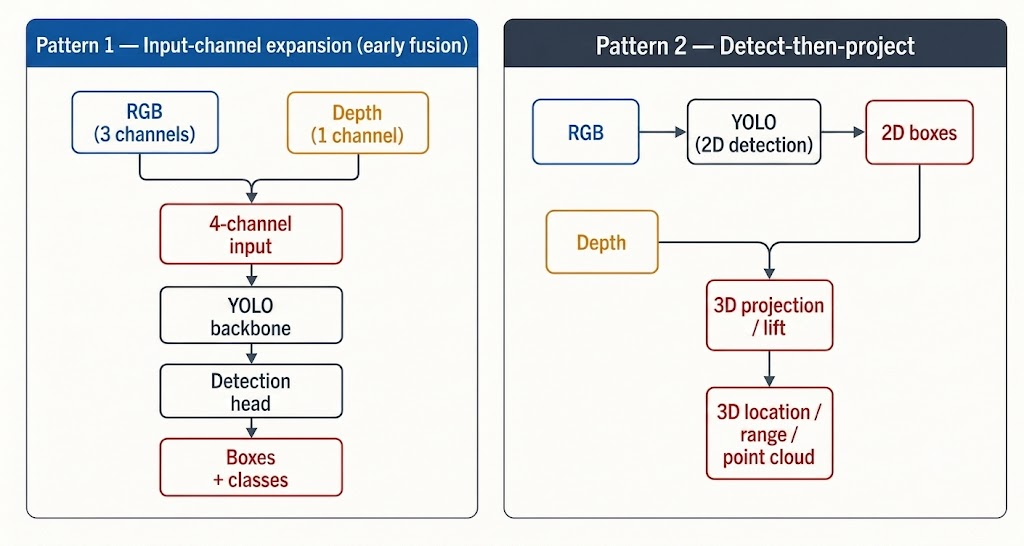
\includegraphics[width=\linewidth]{F05-pola-yolorgbd-gpt-image-2-en}
\caption{The two recurring patterns for integrating YOLO with depth. Pattern one expands the input to four channels and fuses at the input (Expandable YOLO), which Ophoff \textit{et al.}\ find is dominated by intermediate fusion; pattern two detects in 2D and then projects or refines in 3D on a reduced region (FusionVision, YOLOv8-URE).}
\label{fig:yolorgbd}
\end{figure*}

Detection-specific fusion is the part of the corpus closest to the FFB architecture. Ophoff \textit{et al.}\ treated the fusion position not as a fixed design choice but as a free parameter to be swept: they duplicated a 27-layer YOLOv2 into two identical branches (one RGB, one depth) and tested 28 possible fusion locations along the network, finding that middle and late fusion were consistently more competitive than naive early (input-level) fusion on their data \cite{ophoff2019multimodal}. The transferable conclusion is not that a specific layer is optimal for FFBs (datasets and objects differ) but the mechanism-level lesson that separate modality pathways should be preserved long enough for the network to decide which evidence is useful, which is the hypothesis an FFB ablation should test. Expandable YOLO represents the opposite, early-fusion extreme: it appends depth as a fourth input channel to YOLOv3 and adds 3D convolution near the output, keeping the input a single (four-channel) image \cite{takahashi2020expandableyolo}, a cheap baseline worth including because the results of Ophoff \textit{et al.}\ predict that it may underperform. More recent systems abandon the single-network assumption and cascade cheap models, a pattern well suited to a resource-constrained plantation platform. FusionVision chains a fast YOLOv8 detector with FastSAM: detection narrows the search to per-object boxes, segmentation refines masks, and the masks are back-projected to 3D from the RGB-D depth, reconstructing and segmenting objects in 3D without running an expensive model over the whole image \cite{elamraoui2024fusionvision}. DODT runs an ensemble of lightweight detectors in parallel and fuses their outputs for onboard dynamic-object detection and tracking from an RGB-D camera on a small quadcopter, trading single-model peak accuracy for robustness and speed on limited hardware \cite{xu2024onboard}. YOLOv8-URE uses 2D detection as a coarse filter that prunes a point cloud to a small object-relevant subset before 3D registration refines the pose for grasping in stacked scenes, the ``detect in 2D, localize in 3D on a reduced set'' pattern that recurs throughout the 3D and pose literature \cite{yang2025yolov8ure}. The broader design space is organized by Feng \textit{et al.}, whose survey classifies multimodal detection and segmentation for autonomous driving along the three axes of what to fuse, when to fuse, and how to fuse \cite{feng2021multimodalsurvey}, and PointNet supplies the permutation-invariant point-set backbone, processing each point by a shared MLP then aggregating with a symmetric function, that underlies much of the 3D branch discussed next \cite{qi2017pointnet}. Taken together, this sub-literature makes a defensible FFB hypothesis concrete: a feature-level or late-fusion detector with an explicit RGB fallback when a depth-quality signal is poor, evaluated against an RGB-only baseline and an early-fusion baseline at matched resolution and hardware, not the untested claim that adding depth necessarily improves detection. The two recurring YOLO+RGB-D integration patterns, input-channel expansion versus detect-then-project, are contrasted in Figure~\ref{fig:yolorgbd}, and Table~\ref{tab:fusion} enumerates the fusion alternatives together with the specific failure mode each must be tested against.

\begin{table}[t]
\centering\small
\caption{Fusion alternatives to be evaluated on the same FFB data.}
\label{tab:fusion}
\begin{tabular}{p{0.16\linewidth}p{0.32\linewidth}p{0.33\linewidth}}
\toprule
Strategy & Potential value & Failure mode to test \\
\midrule
Early fusion & Minimal architectural change; may exploit aligned low-level cues & Raw depth noise or scale mismatch can contaminate RGB features. \\
Feature fusion & Lets each modality form task-specific features before exchange & Fusion scale and alignment become hyperparameters; extra compute must be justified. \\
Late fusion & Supports a strong RGB fallback and explicit confidence weighting & May miss fine complementary cues needed to separate crowded instances. \\
Cross-modal attention / gating & Can select or suppress modality evidence by context & Attention is not a guarantee of robustness; missing-depth and sunlight ablations are required. \\
\bottomrule
\end{tabular}
\end{table}



\subsection{Multimodal evidence beyond RGB-D (2015--2026)}

The corpus also contains RGB-thermal pedestrian perception, remote sensing, medical imaging, and industrial inspection. These areas must not be merged with agricultural evidence, but they expose recurring multimodal and small-object questions and repeatedly show that concatenation is an assumption about calibration.

RGB-thermal pedestrian detection is the corpus's cleanest study of confidence-aware fusion under changing illumination, which is the FFB problem of deep shadow versus direct sunlight in a different guise. The KAIST benchmark made the enabling hardware choice, using an optical beam-splitter rig to align RGB and thermal pixel-for-pixel at capture time rather than correcting misalignment afterward \cite{hwang2015kaist}, a reminder that paired-modality registration is a data-collection decision, not only an algorithmic one, and it applies to how an FFB RGB-D rig must be built. IAF R-CNN then made the key mechanistic observation that the reliability of each modality depends on illumination: it estimates a scalar illumination value for the image through a small sub-network and uses it to weight the RGB and thermal branches per image, so the model leans on thermal at night and RGB by day \cite{li2019illumination}. MBNet argued that fusing only at the score level is too late and injected a differential modality-aware signal at each convolutional stage, plus alignment, to address the imbalance where one modality dominates \cite{zhou2020mbnet}. CFR replaced a single fusion step with a cycle of fuse-and-refine blocks, iterating the combination several times so the modalities progressively correct each other \cite{zhang2020cfr}, and GAFF staged the fusion into intra-modal attention (highlighting informative regions within each modality) followed by inter-modal attention (weighting one modality against the other) \cite{zhang2021gaff}. CFT posed RGB-thermal fusion as self-attention over a single joint token sequence inside a two-branch YOLOv5, so every RGB token can attend to every thermal token directly \cite{fang2022cft}. A method that exploits thermal contrast at night does not establish that RGB-D helps under tropical sunlight, but this lineage supplies the illumination-conditioned and modality-imbalance ablations an FFB study must run before claiming a depth gain.

Remote sensing is the corpus's small-object and high-resolution laboratory, and a distant bunch under a moving platform is a small object. YOLT tiled huge satellite images spatially and tuned the detector's internal resolution rather than downscaling the image, so tiny objects survive \cite{vanetten2018yolt}. TPH-YOLOv5 added a fourth high-resolution prediction head (P2) and a transformer prediction head to YOLOv5 for drone imagery to recover the small objects that dominate aerial scenes \cite{zhu2021tphyolov5}. UAV-YOLOv8 combined BiFormer dynamic attention, which suppresses irrelevant background in the backbone, with efficient partial convolution to strengthen micro-object representation \cite{wang2023uavyolo}, and RiO-DETR extended the real-time DETR framework to oriented object detection by decoupling angle handling from position across the query representation, attention, and matching \cite{hu2026riodetr}. These small-object and orientation techniques are candidate modifications for detecting distant, variably-oriented bunches.

Medical and industrial inspection show the same general detector specialized into high-stakes, defect-sensitive domains, demonstrating both how to adapt YOLO and why generic numbers do not transfer. In medicine, a single-stage YOLO predictor performed simultaneous COVID-19 lesion detection and classification directly from full-resolution chest X-rays \cite{alantari2020covid}; a YOLO-based decision-level fusion combined several class-specialized YOLOv3 models to trade off the high sensitivity of single-class models against the flexibility of a multi-class one for breast-lesion detection \cite{baccouche2021breast}, a fusion-of-specialists idea transferable to distinct maturity classes; and a systematic review synthesized 124 medical YOLO studies into a taxonomy of clinical modality, YOLO architecture, and task, quantifying how pervasively the family has been adapted \cite{qureshi2024medyolo}. In industry, a comparative study transfer-learned the YOLOv5 s/m/l/x variants for safety-helmet detection and mapped which variant best fits a real deployment \cite{zhou2021helmet}; EFC-YOLO redesigned YOLOv7's feature processing with a Fusion-Faster module to reduce spatial redundancy while preserving defect-position information on steel strips \cite{yang2023efcyolo}; and PCB-YOLO enhanced YOLOv8n with coordinate attention and multi-scale fusion to catch tiny printed-circuit-board defects while cutting parameters \cite{tang2024pcbyolo}. The recurring lesson across medicine and industry is that a general detector is routinely re-tuned to a domain's specific object scale and failure costs, the exact adaptation an FFB detector requires, which is also why a COCO or VOC number cannot be read as an expected plantation result.

\subsection{Benchmark datasets (2012--2020)}

Benchmark data determine what a model can learn and what a score can mean, and the six datasets in the corpus explain both why the transferable methods above exist and why none of them is a substitute for a plantation benchmark. NYU Depth v2 recorded 1{,}449 densely annotated indoor RGB-D images from 464 scenes with a Kinect, adding not only per-pixel class labels but instance numbers and physical support relations, which made structured indoor understanding learnable for the first time \cite{silberman2012nyu}. SUN RGB-D assembled 10{,}335 RGB-D images from several modern depth sensors and improved the raw, hole-ridden depth maps, providing scene-understanding annotations at scale \cite{song2015sunrgbd}, and ScanNet paired cheap consumer-sensor acquisition with an automated server-side reconstruction pipeline and staged crowdsourced labelling to deliver 1{,}513 richly annotated 3D reconstructions from 2.5M RGB-D frames \cite{dai2017scannet}, a template for scaling annotation that an FFB dataset effort could borrow. The whole RGB-D dataset landscape was itself catalogued by Lopes \textit{et al.}\ through backward-snowballing to trace every public release \cite{lopes2022rgbddatasets}. On the generic-detection side, Microsoft COCO shifted recognition from isolated objects toward objects-in-context with 328{,}000 images and instance masks, and it remains the standard source of detection pretraining weights and the AP vocabulary used throughout this review \cite{lin2014coco}. For outdoor perception under a moving platform (the condition closest to a ground vehicle in a plantation), KITTI was the first calibrated multi-sensor outdoor benchmark, capturing synchronized stereo, LiDAR, and localization from a moving car \cite{geiger2012kitti}, and nuScenes extended this to a 360-degree multimodal suite of six cameras, one LiDAR, and five radars over 1{,}000 driving scenes with no blind spot \cite{caesar2020nuscenes}. Every one of these supports pretraining, depth-registration sanity checks, and controlled ablations, but their indoor geometry or urban-driving context, their sensors, and their object categories differ materially from an oil-palm canopy. None substitutes for a plantation dataset whose visual context, target size, maturity labels, camera trajectory, and sensor failures are themselves part of the scientific question. The corollary for evaluation is strict: splits must separate whole trees, traversal sequences, or collection sessions, and a stronger external test must separate sites, days, sensor settings, and lighting regimes, because randomly mixing frames from one video lets a model memorize background, illumination, or even the same bunch seen from a nearby view.



\subsection{Agricultural transfer and the boundary of current evidence (2016--2026)}

The orchard counting studies were examined in Section~\ref{sec:orchard}. This subsection turns to the direct oil-palm evidence and asks which of the steps in Table~\ref{tab:mechanisms} it has measured.

\subsubsection{Oil-palm detection, classification, and datasets}

The direct oil-palm literature has concentrated on the grade of a single bunch. Lai \textit{et al.}\ reviewed ripeness-detection methods across sensing families, and Goh \textit{et al.}\ reviewed non-destructive classification by computer vision, LiDAR, spectroscopy, thermal sensing, and laser-light backscatter \cite{lai2023palmslr,goh2025palmreview}. Both treat sensor choice and class definition as the central problems. Several primary studies show why. Hashim \textit{et al.}\ scanned under-ripe, ripe, and over-ripe bunches with a LiDAR and related the relative reflectance intensity to ripeness \cite{ledger_r_97003608b250cdc5}. Phimpisan and Chungchoo excited 100 Tenera bunches (80 ripe, 20 under-ripe) with ultraviolet LEDs at 395--400~nm in darkness and classified them from the fluorescence image, agreeing fully with five experts and with laboratory oil-content measurements \cite{ledger_r_1c81e223679e4bfe}. Shiddiq \textit{et al.}\ photographed the front and back of 20 Dura and 20 Tenera bunches and found that fruitlet count, fruitlet density, and RGB intensity differed between the two varieties, an attribute that mills must check because only a limited share of Dura is accepted \cite{ledger_r_722bfce242f37ecb}. These studies establish that maturity is not the only class attribute an inventory may need, and that the most reliable measurements so far were made under controlled light on one bunch at a time.

The camera-based detection studies moved to plantation imagery. Lai \textit{et al.}\ detected ripe bunches with YOLOv4 and an Intel RealSense D435 RGB-D camera, reaching an mAP of 87.9\% at 21 FPS \cite{lai2022yolov4palm}. Mansour \textit{et al.}\ compared MobileNetV2-SSD, three EfficientDet-Lite models, and three YOLOv5 sizes on four classes (ripe, unripe, half-ripe, and over-ripe), noting that the surface changes from black or dark purple when unripe to dark red when ripe; YOLOv5m was best, with an mAP$_{50{:}95}$ of 0.842 \cite{ledger_r_19d96439ecdda18d}. Sabillah \textit{et al.}\ compared YOLOv3, v4, v7, and v8 and found YOLOv8 best \cite{ledger_r_134385f2faed38a6}, and Naftali \textit{et al.}\ proposed a depthwise-separable YOLOv8 variant as a real-time counter \cite{naftali2024palmcounter}. Chen \textit{et al.}\ reported a YOLOv4 mAP of 98.5\% on a small set of images collected from Kaggle and Google, without field or multi-view validation \cite{chen2022ffbdet}. These results support the choice of a YOLO-family detector for the M0 step. None of them measures whether a bunch found in one image is the bunch found in another.

The only oil-palm counting study in the evidence register counted bunches on a conveyor, not on a tree. Shiddiq \textit{et al.}\ recorded 117 Tenera bunches moving past an RGB camera at 20 FPS, detected them with an HSV colour rule, and tracked them between frames \cite{shiddiq2023palmcount}. The best video was counted without error, but the average accuracy over ten videos was 79.35\%. The failures had a physical cause: when a bunch lay with its darker side toward the camera, the colour rule missed it, and accuracy depended on room lighting. The same dark surface is characteristic of the least mature class in SawitMVC, which has the lowest AP50 in the published baseline \cite{indriani2026sawitmvc}.

Two dataset papers expose acquisition variables that the design space needs. Goh \textit{et al.}\ released 400 RGB images from a 50-megapixel smartphone sensor and 400 registered depth maps and point clouds from an Intel RealSense D455f, collected at four plantation locations in Johor under varied illumination, angle, and distance \cite{goh2025palmdataset}. Ripeness is binary and follows Malaysian Palm Oil Board standards; the RGB-depth registration error is 1.8~cm at 3~m, and expert inter-rater agreement is 92.5\%. It is the first public oil-palm dataset in the register that pairs field RGB with sensor depth. Suharjito \textit{et al.}\ released plantation images taken from multiple angles with five categories: unripe, under-ripe, ripe, flower, and abnormal \cite{suharjito2025palmdataset}. Neither dataset makes the identity of a bunch across views an annotated quantity.

SawitMVC does. Its 953 trees were photographed with smartphones at two commercial plantations in South Kalimantan from four or eight positions around the trunk; boxes carry four BBC maturity classes, and a per-tree JSON layer links the boxes of each physical bunch across views into 9{,}823 unique bunches, split by tree into 716 training, 96 validation, and 141 test trees \cite{indriani2026sawitmvc}. The authors state that no other public oil-palm dataset provides a per-tree count of unique bunches that is independent of detector output. The dataset therefore supports all three evaluations that the orchard studies separated: detection, count, and the association between them. Its limitations are also stated: two plantations, one collection period in February 2026, and no depth channel.

Remaining oil-palm studies address other scales or sensors: UAV structure from motion for canopy height and per-palm inventories \cite{ledger_m_084cfd5badbb63d3}, LiDAR mapping of bunch distribution \cite{ledger_r_3e45c6dc2566f46b}, and colour features for real-time maturity grading \cite{ledger_r_2f7d604b1d3fa5e4}. In every case the output is per-image or per-bunch detection or classification; none reports a tree-level count with cross-view deduplication.





\subsubsection{Positioning against previous reviews}

Six prior reviews address adjacent rather than identical questions. Table~\ref{tab:position} records their stated scope and identifies whether cross-view identity is treated as the primary unit. The wording is deliberately bounded: ``not explicit'' means that the accessible scope and abstract do not make identity and duplicate rejection the central organizing question.

\begin{table}[t]
\centering
\caption{Positioning against previous reviews.}
\label{tab:position}
\scriptsize
\begin{tabularx}{\columnwidth}{@{}p{0.24\columnwidth}p{0.22\columnwidth}p{0.14\columnwidth}Y@{}}
\toprule
Review & Primary scope & Cross-view identity? & Position\\
\midrule
Lai et al.~\cite{lai2023palmslr} & FFB ripeness detection & Not explicit & Sensor context; does not organize counting mechanisms.\\
Goh et al.~\cite{goh2025palmreview} & FFB classification, non-destructive sensors & Not explicit & Modality limits; this review adds identity evaluation.\\
Naftali et al.~\cite{naftali2024palmcounter} & FFB detector comparison & Not explicit & Detector context; this review separates detection from inventory.\\
Naghipour et al.~\cite{naghipour2024fruitreview} & AI for fruit detection & Not explicit & Broad coverage; this review makes association a design axis.\\
Alif and Hussain~\cite{sapkota2024yoloagri} & YOLO in agriculture & Not explicit & Architecture taxonomy; this review is task-first.\\
Nordin and Misro~\cite{nordin2026palmslr} & Palm-oil maturity, deep learning & Not explicit & Maturity comparator; this review generalizes the class attribute.\\
\bottomrule
\end{tabularx}
\end{table}

The bounded conclusion is not ``no previous review exists.'' It is that the accessible review set is organized mainly by sensor, ripeness, detector family, or agricultural application. The cross-view identity of each physical fruit as the prerequisite for a class-wise inventory is not the primary comparison unit in that set. This is the gap addressed here.



\subsection{Research priorities for field evaluation}
\label{sec:agenda}

\begin{figure*}[t]
\centering
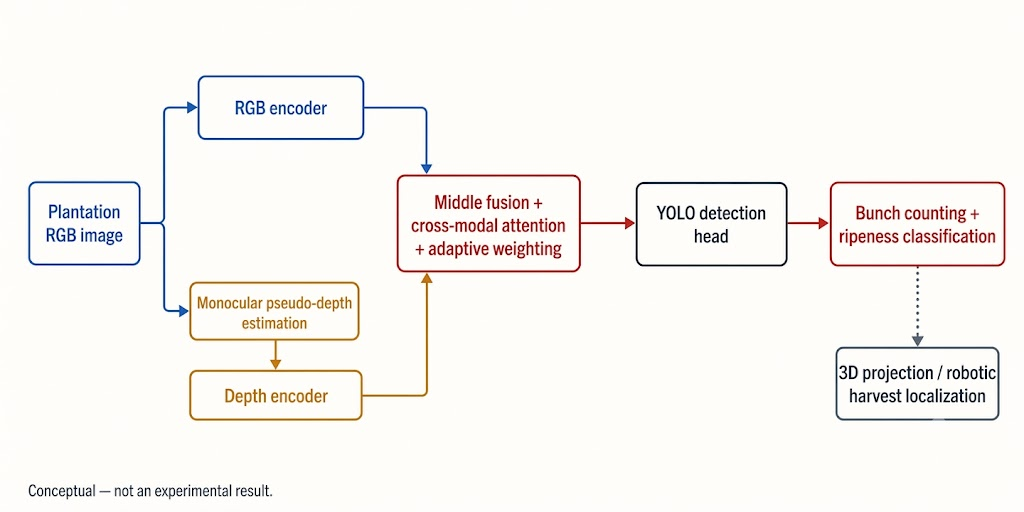
\includegraphics[width=\linewidth]{F08-pipeline-sawit-gpt-image-2-en}
\caption{Conceptual pipeline implied by the evidence map: a plantation RGB image feeds an RGB encoder and, in parallel, a depth branch whose source (monocular prediction or calibrated sensor) must be declared; quality-aware fusion feeds a real-time detector; per-instance maturity, an instance-constrained depth sample, and pose-based temporal association then produce a de-duplicated bunch inventory. Every stage is a hypothesis corresponding to one ablation in the agenda below, not a validated component.}
\label{fig:pipeline}
\end{figure*}

The evidence map points to a testable program rather than a claimed final architecture. Figure~\ref{fig:pipeline} makes the required stages and their dependencies explicit. First, construct a paired RGB-D FFB dataset with calibration metadata and annotations for bunch instances, maturity, occlusion, apparent size, illumination, depth validity, and where possible cross-frame identity. Reference counts must be collected at an operational unit such as a tree, short row, or traversal, because frames alone cannot validate a counting system, and splits must separate trees, sequences, and sessions to prevent optimistic transfer.

Second, establish an RGB-only YOLO baseline and one high-capacity comparison such as a two-stage, instance-segmentation, or transformer detector. Third, compare early fusion, at least one feature-fusion configuration, late fusion, and a depth-quality-gated RGB fallback, all under the same split, resolution, annotation policy, and target hardware. The core comparison is causal: does the added depth branch improve a stated failure mode enough to justify its sensor and latency cost?

Fourth, evaluate at the four levels of Table~\ref{tab:metrics}: detection stratified by size and occlusion; per-instance maturity with calibration reported by illumination; geometry that names whether a prediction is relative depth, calibrated range, or 3D position; and counting with absolute and signed error, duplicate rate, and association quality per sequence. Report latency, memory, and depth status with every accuracy table. Finally, perform failure-oriented ablations: remove depth deliberately, introduce missing or noisy depth, vary RGB-D alignment, compare shaded and sunlit frames, and test both stationary and moving camera sequences. If an RGB fallback matches or exceeds a fusion configuration whenever depth quality is poor, that is a meaningful deployment finding, not a negative result.



\section{Synthesis, Discussion, and Limitations}
\label{sec:synthesis}

\subsection{Synthesis}

\begin{figure*}[t]
\centering
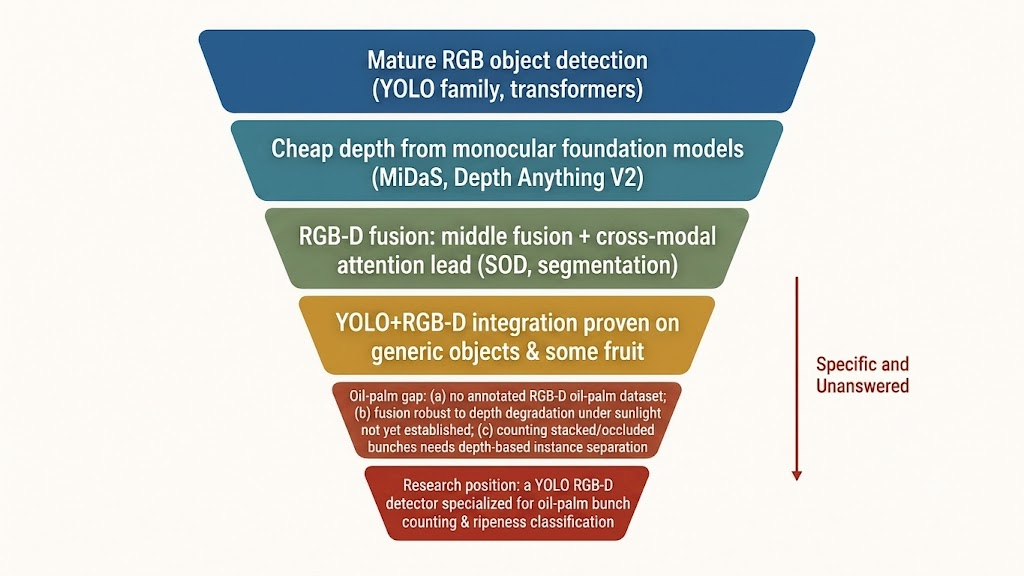
\includegraphics[width=\linewidth]{F07-funnel-sawit-gpt-image-2-en}
\caption{The evidence funnel that motivates the research agenda. Mature general RGB detection, cheap foundation-model depth, and RGB-D fusion narrow, layer by layer, toward the specific and largely unfilled requirement: a calibrated paired RGB-D benchmark for oil-palm bunch counting and maturity classification.}
\label{fig:funnel}
\end{figure*}

The review began with two failures recorded in one table: duplication, which turns 9{,}823 bunches into 18{,}540 boxes, and detection, which reduces tree-level count accuracy from 88.65\% to 33.33\% when annotated boxes are replaced by predicted ones \cite{indriani2026sawitmvc}. The literature examined since then answers the two unevenly.

For duplication, the orchard studies provide a sequence of mechanisms and a measured failure for each. A statistical correction is repeatable and, on clean boxes, nearly unbiased, but it cannot name the fruit it corrects \cite{ledger_r_408d13511cac4177,indriani2026sawitmvc}. Appearance matching did not improve on motion alone for fruit that look alike \cite{ledger_r_ee550a3e3a6fb318,ledger_r_2d972b94554c6cd1}. Tracking requires a continuous path. Monocular geometry removed most double-counted tracks under heavy occlusion but lacked scale, and it lost fruit where two sides of a tree had to be joined \cite{ledger_m_9966d81433d61ed3,ledger_r_00f82e0f404d691b}. Metric geometry failed where pose drift exceeded the distance between neighbouring fruit \cite{ledger_r_d4270ea8ab11f268}, and 3D clustering under-counted fruit that grow in contact \cite{ledger_m_1210e3ea00486b68}. The transferable literature addresses each of these causes separately: SLAM for drift, metric depth and canonical-camera models for scale, frustum-based 3D localization for placing a detection in space, and confidence-aware decisions for withholding a record. It has not been assembled and tested on oil palm.

For detection, the evidence is weaker. The detector literature explains how instances are formed and how NMS and one-to-one assignment affect crowded scenes, but none of the generations reviewed here has been shown to remove the failure on small, dark, frond-covered bunches. Depth is the candidate that the multimodal literature offers, and its value is conditional. The fusion studies agree that depth should be admitted only when its quality has been checked, and they disagree about where it should enter the network. Figure~\ref{fig:funnel} depicts the resulting narrowing from mature general vision toward the still-missing calibrated RGB-D benchmark for class-wise FFB inventories. The review therefore treats the literature as a map from mechanisms to testable hypotheses, not as a pool from which to compute an expected accuracy.

\begin{table*}[t]
\centering\small
\caption{Metric hierarchy for a class-wise fruit-inventory study. Each level answers a different question and cannot be replaced by a single AP score.}
\label{tab:metrics}
\begin{tabular}{p{0.20\textwidth}p{0.32\textwidth}p{0.37\textwidth}}
\toprule
Evaluation level & Required measurements & Scientific interpretation \\
\midrule
Detection & AP, precision, recall, size/occlusion/illumination strata & Determines whether instances are visible to the pipeline. \\
Class attribute (maturity as the case here) & Per-instance class metrics, calibration, confusion matrix & Tests whether the right label is attached to the right instance; a per-class count is defined only once that instance is identified. \\
Geometry & Declared coordinate frame, range or position error, valid-depth rate & Establishes what spatial claims are justified. \\
Association and count & Count error, bias, duplicate rate, false merges, association precision/recall & Tests the inventory rather than an isolated frame. \\
Deployment & Latency, throughput, memory, hardware, depth availability & Establishes whether the result is feasible in field operation. \\
\bottomrule
\end{tabular}
\end{table*}

\begin{figure}[t]
\centering
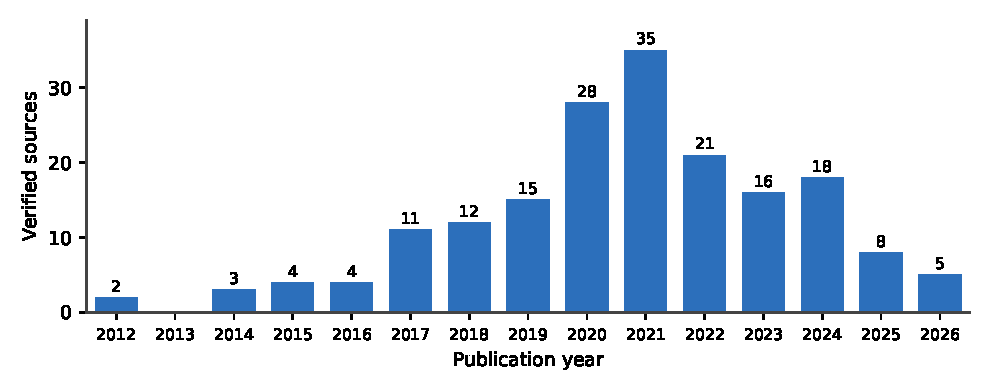
\includegraphics[width=\linewidth]{fig-corpus-year}
\caption{Temporal distribution of the reviewed primary literature by publication year (2012--2026). The peak in 2020--2024 coincides with the parallel maturation of RGB-D fusion, foundation-model monocular depth, and end-to-end detection.}
\label{fig:corpus-year}
\end{figure}

\begin{figure}[t]
\centering
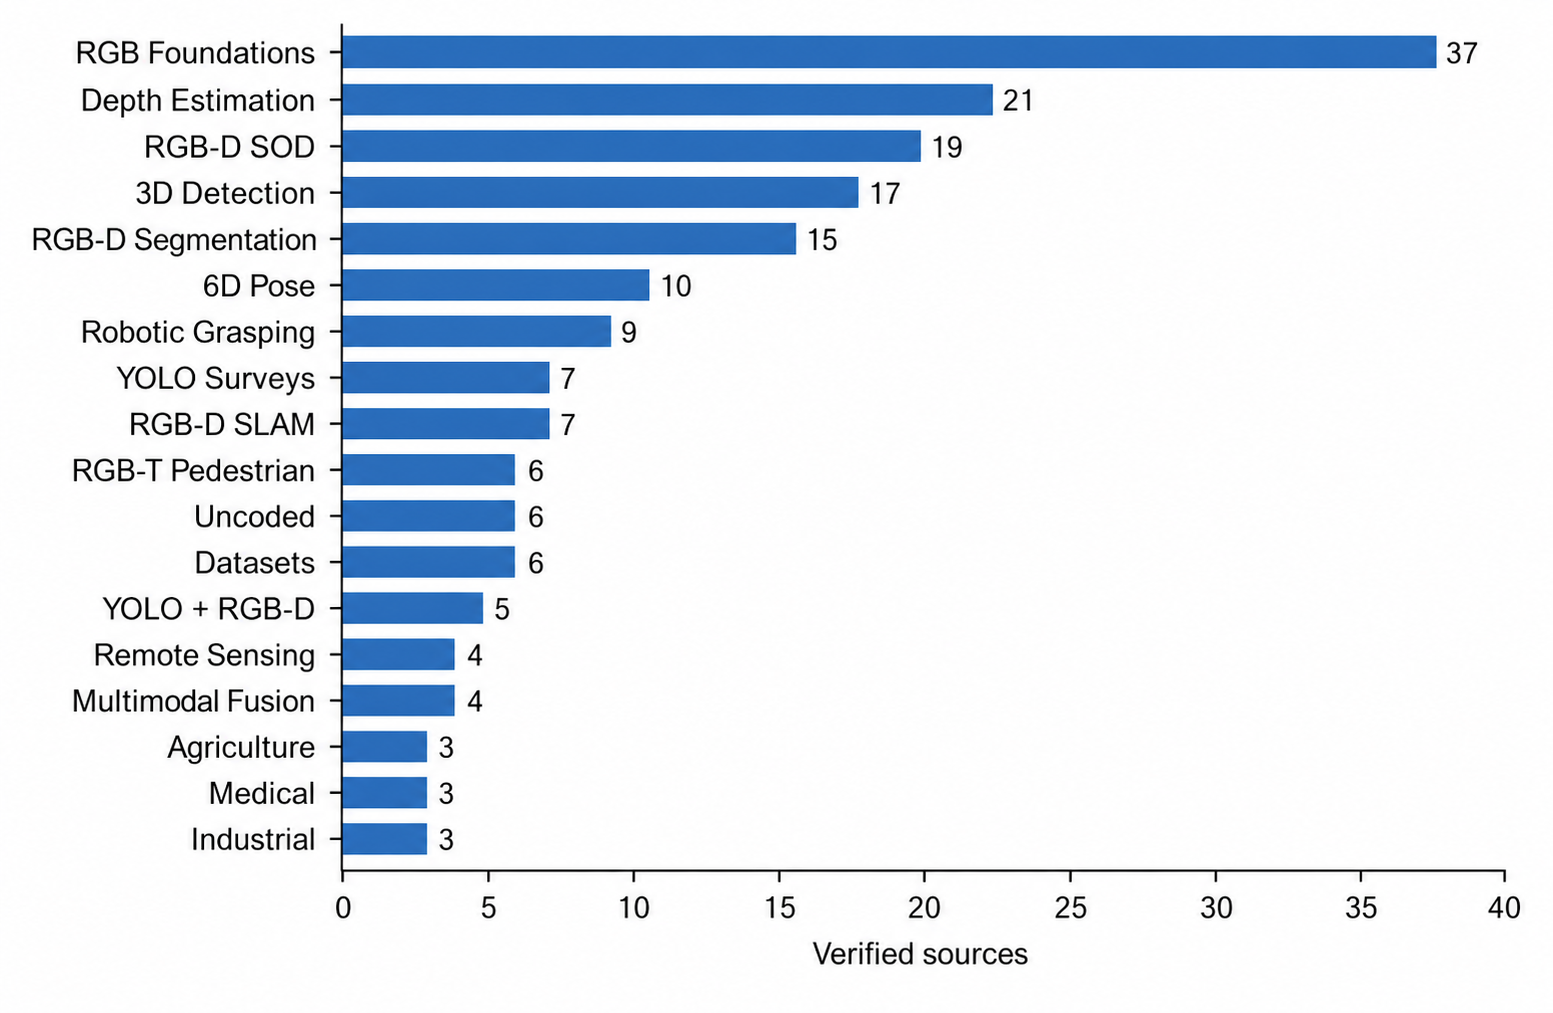
\includegraphics[width=\linewidth]{fig-corpus-theme-gpt-image-2-en}
\caption{Thematic distribution of the reviewed primary literature across the seventeen coded research areas. The concentration in general RGB detection, monocular depth, and RGB-D dense prediction, against limited direct agricultural evidence, defines the transfer gap this review addresses.}
\label{fig:corpus-theme}
\end{figure}

\subsection{Discussion}

The literature supports three bounded conclusions. First, a multi-scale real-time RGB detector is an appropriate baseline for an FFB system, but model choice should follow field latency and error modes. Generic leaderboard rank is not sufficient, because controlled re-training changes the ranking with dataset and model size \cite{alif2024yoloevolution}. Second, an explicit identity mechanism is justified for a four- or eight-position census only if it outperforms the statistical correction that SawitMVC already provides. On annotated boxes that correction is within one bunch per class for 95.57\% of cases \cite{indriani2026sawitmvc}, so the case for M4 or M5 rests on the predicted-box condition, on class-wise attribution, and on the ability to say which bunch was counted. Third, feature-level, late, and quality-aware fusion are justified experimental alternatives because they keep a modality-specific representation and allow an RGB fallback. The evidence does not establish that a particular YOLO generation, depth model, or fusion point is best for oil palm, or that RGB-D produces a numerical gain on FFB. A paired field dataset and controlled ablations are needed to answer those questions.

The sharpest disagreement inside the corpus concerns where depth should enter. Ophoff \textit{et al.}\ swept 28 fusion positions along a two-branch YOLOv2 and found input-level fusion dominated by middle and late fusion \cite{ophoff2019multimodal}, whereas Expandable YOLO appended depth as a fourth input channel to a single backbone \cite{takahashi2020expandableyolo}. D3Net and SA-Gate move the question from position to admission. D3Net showed that a low-quality depth map degrades prediction unless a depurator discards it \cite{fan2020d3net}, and SA-Gate gates each modality with information computed from the other before fusion \cite{chen2020sagate}. No study in the corpus tests these positions on agricultural data, where depth fails in ways that indoor benchmarks do not exercise, including holes and noise under direct sunlight. The oil-palm dataset of Goh \textit{et al.}\ provides registered field depth for binary ripeness \cite{goh2025palmdataset}, and SawitMVC provides cross-view identity without depth \cite{indriani2026sawitmvc}. A dataset with both does not yet exist in the reviewed literature.

\subsection{Limitations}
\label{sec:limitations}

The evidence map is targeted rather than exhaustive. Its database coverage and retrieval constraints may miss relevant work, and metadata records cannot substitute for article-level evidence. The search trace in Appendix~C makes this boundary inspectable without treating the search pool as an included-study count.

The focused evidence matrix mixes direct agricultural studies, fruit studies, transferable mechanism papers, and reviews. This is deliberate for a design-space review, but the evidence classes are not interchangeable. A result from an autonomous-driving benchmark does not establish oil-palm performance. A review that discusses ripeness does not establish cross-view identity. A dataset descriptor establishes the availability of labels and sensors, not the superiority of a model. Several of the orchard failure analyses used here come from single studies on one crop and one site, and their numbers describe those conditions.

The review does not estimate a pooled accuracy, rank all detectors, or claim that explicit deduplication is always beneficial. Its bounded claim is that cross-view identity is a necessary design variable for the stated inventory task and that the value of each identity mechanism should be evaluated under its acquisition assumptions.

\section{Conclusion}

The count of a tree depends on two decisions that current evaluation often merges: whether a bunch is detected in an image, and whether two detections are the same bunch. The SawitMVC baselines show both failures on one test split. A counter that places all four class counts within one bunch of the truth on 88.65\% of trees when given annotated boxes does so on 33.33\% when given the boxes of a current detector, and a naive sum of even perfect boxes does so on 6.38\% of trees \cite{indriani2026sawitmvc}.

A decade of orchard studies has produced mechanisms for the second decision and measured their failures: calibration that cannot name the duplicated fruit, appearance matching that fails for look-alike fruit, monocular geometry without scale, and metric geometry defeated by pose drift in turns. Each failure has a counterpart in the transferable literature on tracking, SLAM, depth, and 3D localization, and none of these combinations has been tested on oil palm. For the first decision, depth is a plausible aid for small and occluded bunches, conditional on quality control and on the fusion point, and it offers no evident remedy for the colour ambiguity between adjacent maturity classes. Progress requires field data that record identity, class, depth quality, and repeated observation together, and evaluations that report association and count alongside detection.


\clearpage
\makeatletter
\setcounter{section}{0}
\renewcommand{\thesection}{\Alph{section}}
\renewcommand{\theHsection}{appendix.\Alph{section}}
\@ifclassloaded{IEEEtran}{\onecolumn}{}
\makeatother

\refstepcounter{section}
\label{app:focused}

\begin{center}
\textsc{Appendix A: Focused evidence matrix}
\end{center}

Table~\ref{tab:focused} contains one row per study included after targeted full-text review from the reproducible search. The ``Mech.'' column uses the codes from Table~\ref{tab:mechanisms}. ``Attr.'' indicates whether the study evaluates a class attribute (e.g., maturity, size) at the instance level. ``Dedup'' indicates whether the study explicitly evaluates or performs cross-view duplicate rejection. The complete machine-readable matrix with additional fields is available as supplementary material.

\footnotesize
\setlength{\LTleft}{0pt}
\setlength{\LTright}{0pt}
\setlength{\tabcolsep}{2pt}
\begin{longtable}{@{}>{\raggedright\arraybackslash}p{0.17\textwidth}>{\raggedright\arraybackslash}p{0.13\textwidth}>{\raggedright\arraybackslash}p{0.07\textwidth}>{\raggedright\arraybackslash}p{0.04\textwidth}>{\raggedright\arraybackslash}p{0.04\textwidth}>{\raggedright\arraybackslash}p{0.37\textwidth}>{\raggedright\arraybackslash}p{0.06\textwidth}@{}}
\caption{Focused evidence matrix. Mechanism codes follow Table~\ref{tab:mechanisms}. Attr.\ = class attribute evaluated; Dedup = duplicate rejection evaluated or performed.}\label{tab:focused}\\
\toprule
Study & Target, sensor & Mech. & Attr. & Dup. & Key finding and limitation & Type\\
\midrule
\endfirsthead
\multicolumn{7}{c}{\tablename\ \thetable{} continued}\\
\toprule
Study & Target, sensor & Mech. & Attr. & Dup. & Key finding and limitation & Type\\
\midrule
\endhead
\midrule
\multicolumn{7}{r}{Continued on next page}\\
\endfoot
\bottomrule
\endlastfoot

Von Hirschhausen et al.\ (2025) \cite{ledger_m_3f8f02033fe9db3a}
& Apple, calibrated stereo RGB
& M4 & -- & No
& Stereo dataset supports detection and 3D reconstruction but does not evaluate cross-view unique identity.
& Direct\\

Fusaro et al.\ (2026) \cite{ledger_r_0eda6374aaf85fae}
& Strawberry, LiDAR point cloud
& M2--4 & -- & Yes
& Learned descriptors and attention-based matching improve temporal fruit re-identification; limited to strawberry annotations.
& Direct\\

Bargoti and Underwood (2016) \cite{ledger_r_143d70deec8d2b1d}
& Apple, monocular RGB UGV
& M0 & -- & No
& CNN segmentation achieves detection F1 0.858 and row-yield $R^2$ 0.826; no persistent identity across views.
& Direct\\

Stein et al.\ (2016) \cite{ledger_r_408d13511cac4177}
& Mango, RGB + GPS/INS + LiDAR
& M3/M4 & -- & Yes
& Multi-view tracking with epipolar geometry yields near-unity calibration slope and 1.36\% over-count on 16 trees.
& Direct\\

Liu et al.\ (2018) \cite{ledger_m_9966d81433d61ed3}
& Orange/apple, monocular video + SfM
& M3/M4 & -- & Yes
& 3D reconstruction correction substantially reduces duplicate and outlier tracks; depends on illumination and camera stability.
& Direct\\

Hashim et al.\ (2018) \cite{ledger_r_97003608b250cdc5}
& Oil palm, LiDAR 905\,nm intensity
& M0 & Mat. & No
& LiDAR intensity separates three FFB ripeness levels; no classification accuracy or cross-view metric.
& Direct\\

Fawcett et al.\ (2019) \cite{ledger_m_084cfd5badbb63d3}
& Oil palm, UAV RGB SfM
& M4 & Size & Yes
& UAV canopy-height models support per-palm inventories; tree-canopy study, not fruit-level identity.
& Direct\\

Liu et al.\ (2019) \cite{ledger_r_00f82e0f404d691b}
& Mango, monocular RGB video
& M3/M4 & -- & Yes
& Monocular tracking + semantic SfM + depth filtering achieve tree-level counts; undercounting increases with occlusion.
& Direct\\

H\"ani et al.\ (2020) \cite{ledger_r_1358c0868a62c84a}
& Apple, RGB image sequences
& M3/M4 & -- & Yes
& Merged CNN counting reaches 95.6--97.8\% of harvest ground truth; inventory quality depends on detection + tracking + geometric merging composition.
& Direct\\

Alfatni et al.\ (2020) \cite{ledger_r_2f7d604b1d3fa5e4}
& Oil palm, controlled RGB CCD
& M0 & Mat. & No
& ANN histogram achieves 94\% maturity grading on conveyor; controlled setting, no multi-view inventory.
& Direct\\

Husin et al.\ (2021) \cite{ledger_r_3e45c6dc2566f46b}
& Oil palm, LiDAR point cloud
& M4 & Mat. & No
& LiDAR maps link FFB to spatial coordinates; no cross-view association or accuracy metric.
& Direct\\

Lai et al.\ (2022) \cite{lai2022yolov4palm}
& Oil palm, RGB-D RealSense D435
& M0 & Mat. & No
& YOLOv4 achieves mAP 87.9\% for ripe FFB detection at 21 FPS; no cross-frame identity.
& Direct\\

Mansour et al.\ (2022) \cite{ledger_r_19d96439ecdda18d}
& Oil palm, RGB ground images
& M0 & Mat. & No
& YOLOv5m achieves mAP$_{50{:}95}$ 0.842 on ground FFB; COVID-restricted dataset, no multi-view evaluation.
& Direct\\

Sun et al.\ (2022) \cite{ledger_r_1a70fa2aeed54ea3}
& Apple, RGB nighttime
& M0 & -- & No
& Nighttime detection AP 85.2\%; no tracking, no cross-view identity.
& Direct\\

Lu et al.\ (2022) \cite{ledger_r_2828a3937318ca86}
& Citrus, RGB handheld
& M0 & -- & No
& Improved Mask R-CNN AP$_{50}$ 95.4\% for green-fruit detection; no temporal or cross-view evaluation.
& Direct\\

Wan Nurazwin et al.\ (2022) \cite{ledger_r_3f230a23a2a956c8}
& Pineapple, UAV top-view RGB
& M0 & -- & No
& ANN counting achieves 94.4\% on 20 sample images; no cross-view deduplication.
& Direct\\

Yang et al.\ (2022) \cite{ledger_r_4b3d8d423dbd5d0e}
& Vehicle, RGB multi-camera
& M2 & -- & N/A
& Weakly supervised cross-view embeddings reduce viewpoint variation; transferable mechanism, not agricultural data.
& Transfer\\

Zhang et al.\ (2022a) \cite{ledger_r_c79d61a639a09929}
& Apple, UAV + ground SfM
& M4 & -- & No
& Complementary UAV and ground point clouds improve coverage; no persistent fruit identity or deduplication.
& Direct\\

Zhang et al.\ (2022b) \cite{ledger_r_ee550a3e3a6fb318}
& Citrus, RGB video rover
& M3 & -- & Yes
& Counting-region strategy with tracking achieves MAE 0.081; track IDs are local to each sequence.
& Direct\\

Chen et al.\ (2022) \cite{chen2022ffbdet}
& Oil palm, RGB online images
& M0 & -- & No
& YOLOv4 mAP 98.5\% on small dataset; Kaggle/Google-sourced images, no field or multi-view validation.
& Direct\\

Phimpisan and Chungchoo (2023) \cite{ledger_r_1c81e223679e4bfe}
& Oil palm, UV fluorescence
& M0 & Mat. & No
& Fluorescence classifies FFB ripeness rapidly; controlled dark-chamber setup, no field multi-view use.
& Direct\\

Gené-Molá et al.\ (2023) \cite{ledger_r_2d972b94554c6cd1}
& Apple, Kinect Azure RGB-D / video
& M3 & -- & Yes
& ByteTrack HOTA 0.689, yield MAPE 7.47\%; appearance ReID did not help visually similar apples.
& Direct\\

Shiddiq et al.\ (2023) \cite{shiddiq2023palmcount}
& Oil palm, RGB video conveyor
& M3 & -- & No
& Conveyor counting mean accuracy 79.4\%; postharvest setup, sensitive to illumination and orientation.
& Direct\\

Rapado-Rincón et al.\ (2023) \cite{ledger_r_700d34dae0f20d78}
& Tomato, RGB + LiDAR robot arm
& M3/M4 & -- & Yes
& Multi-view perception recovers occluded fruit; HOTA up to 71.5\%, MAPE 12.2\%. Count error alone hides ID switches.
& Direct\\

Abeyrathna et al.\ (2023) \cite{ledger_r_9e1316b934e66409}
& Apple, RGB-D RealSense + tractor
& M3 & -- & Yes
& Deep SORT with depth prevents repeated counting; artificial orchard with 30 apples on 10 trees.
& Direct\\

Hu et al.\ (2023) \cite{ledger_r_d594d85dc382f9ff}
& Apple, RGB video
& M3 & -- & Yes
& SURF + Kalman cascade tracking reduces repeated counts vs SORT; three test videos, no full identity metric.
& Direct\\

Lai et al.\ (2023) \cite{lai2023palmslr}
& Oil palm, multi-sensor review
& M0 & Mat. & N/A
& Review covers ripeness and detection; does not formulate cross-view identity or unique inventory as a problem.
& Direct\\

James et al.\ (2023) \cite{ledger_r_fd5751e2ca2f7496}
& Citrus, RGB ground images
& M0 & -- & No
& Public citrus benchmark with 44,233 boxes; front/back aggregation does not establish unique fruit identity.
& Direct\\

Lin et al.\ (2024) \cite{ledger_r_1c69e46dac45d45d}
& Citrus, RGB ground images
& M0 & -- & No
& AG-YOLO mAP$_{50}$ 83.2\% under severe occlusion; single-view benchmark, no cross-view identity.
& Direct\\

Ambrus et al.\ (2024) \cite{ledger_r_3e129b7285059b95}
& Tomato, DSLR + robot RGB + 3D scan
& M0/M4 & Mat. & No
& Robot/DSLR + 3D shape supports count and weight estimation; one-sided views cause missed fruit.
& Direct\\

V\'elez et al.\ (2024) \cite{ledger_r_659a7da54b8a43e6}
& Grape, smartphone + UAV + RTK
& M4 & -- & N/A
& Geospatial anchors align multi-source data at plant level; no individual fruit identity.
& Transfer\\

Wu et al.\ (2024) \cite{ledger_r_92ac7cb4b797197d}
& Apple, RGB orchard + synthetic fog
& M0 & -- & No
& Lightweight detector mAP$_{50}$ 94.3\% across weather conditions; no tracking or cross-view identity.
& Direct\\

Vidhya and Priya (2024) \cite{ledger_r_e8d88a31640ee300}
& Mango, RGB mobile camera
& M0 & -- & No
& YOLOv7 mAP$_{50}$ 99.5\% reported on training/validation; no separate test or cross-view metrics.
& Direct\\

Hobart et al.\ (2025) \cite{ledger_m_66042c905cc191de}
& Apple, UAV RGB SfM + RTK
& M4 & -- & No
& SfM recovers ripe-apple 3D positions for yield-mass mapping; no persistent fruit identity.
& Direct\\

Montalb\'an Faet et al.\ (2025) \cite{ledger_m_949f38a7336860d8}
& Citrus, UAV RGB + multispectral
& M4 & -- & No
& Cross-spectral annotations with date-based split; data article without detector benchmark.
& Direct\\

Dutta et al.\ (2025) \cite{ledger_m_dcfc5d3cb912146d}
& Apple, UAV + ESP32-CAM edge
& M0 & -- & No
& Low-cost edge pipeline for detection; temporal consistency identified as future work.
& Direct\\

Sabillah et al.\ (2025) \cite{ledger_r_134385f2faed38a6}
& Oil palm, RGB smartphone + UAV
& M0 & -- & No
& YOLOv8 mAP 99.0\%; small dataset, no independent test split or multi-view evaluation.
& Direct\\

Goh et al.\ (2025) \cite{goh2025palmdataset}
& Oil palm, RGB-D RealSense + point cloud
& M4 & Mat. & No
& 400 RGB-depth-point-cloud scenes with calibration; data article, no detector benchmark or cross-session identity.
& Direct\\

Timprae et al.\ (2025) \cite{ledger_r_4d09eb83eea41b2f}
& Tomato, RGB handheld + SfM/NeRF
& M4 & Mat. & No
& Instance segmentation + SfM + DBSCAN + ellipsoid fitting for phenotyping; manual intervention still required.
& Direct\\

Hamid et al.\ (2025) \cite{ledger_r_504a1d386928344f}
& Oil palm, multi-sensor review
& M0 & Mat. & N/A
& Mini-review on ripeness; narrative format, no reproducible search or cross-view analysis.
& Direct\\

Shiddiq et al.\ (2025) \cite{ledger_r_722bfce242f37ecb}
& Oil palm, RGB CMOS conveyor
& M0 & Mat. & No
& Front/back ImageJ counts are lower than manual due to overlapping fruitlets; no cross-view registration.
& Direct\\

Lee et al.\ (2026) \cite{ledger_r_d4270ea8ab11f268}
& Pear, RGB + LiDAR + SLAM
& M3/M4 & -- & Yes
& 96.2\% counting accuracy with LiDAR--camera fusion; 53 double-counts remain from threshold and SLAM drift.
& Direct\\

Meyer et al.\ (2024) \cite{ledger_m_1210e3ea00486b68}
& Fruit (synthetic + apple), RGB multiview NeRF
& M4 & -- & Yes
& Semantic NeRF clusters fruit in 3D, addressing duplicate counting; sensitive to sparse views and hyperparameters.
& Direct\\

Wang et al.\ (2025) \cite{ledger_r_b2e0e9aabad17a97}
& Tomato, RGB-D + ORB-SLAM3
& M4 & Size & No
& RGB-D SLAM projects segmentation into 3D for per-plant count and volume; leaf occlusion and depth errors cause missed fruit.
& Direct\\

\end{longtable}

\clearpage
\makeatletter
\@ifclassloaded{IEEEtran}{\twocolumn}{}
\makeatother


\refstepcounter{section}
\label{app:queries}
\begin{center}
\textsc{Appendix B: Exact search strings}
\end{center}

\subsection*{Q1: Multi-view fruit inventory}
\begin{verbatim}
TITLE-ABS-KEY(("fruit" OR "fresh fruit
bunch" OR "FFB" OR "oil palm" OR "apple"
OR "citrus" OR "mango" OR "grape" OR
"berry" OR "bunch" OR "cluster" OR "crop")
AND ("count*" OR "yield estimation" OR
"load estimation" OR "fruit load" OR
"inventory" OR "enumeration")
AND ("multi-view" OR "multiple view*" OR
"multi-camera" OR "video" OR "cross-view"
OR "structure from motion" OR "SfM" OR
"track*" OR "3D reconstruction" OR
"image sequence"))
AND PUBYEAR > 2014 AND PUBYEAR < 2027
AND (SUBJAREA(AGRI) OR SUBJAREA(COMP)
OR SUBJAREA(ENGI) OR SUBJAREA(MULT))
\end{verbatim}

\subsection*{Q2: Cross-view identity and duplicates}
\begin{verbatim}
TITLE-ABS-KEY(("multi-view" OR "cross-view"
OR "multi-camera" OR "multiple cameras" OR
"overlapping view*" OR "multi-sensor")
AND ("re-identification" OR
"data association" OR "identity" OR
"duplicate*" OR "deduplicat*" OR
"double counting" OR "correspondence" OR
"instance matching" OR "track*" OR
"association")
AND ("object detection" OR
"instance segmentation" OR "counting" OR
"instance" OR "pedestrian" OR "vehicle"))
AND PUBYEAR > 2014 AND PUBYEAR < 2027
AND (SUBJAREA(COMP) OR SUBJAREA(ENGI)
OR SUBJAREA(AGRI) OR SUBJAREA(MULT))
\end{verbatim}

\subsection*{Q3: Plant geometry and multimodal sensing}
\begin{verbatim}
TITLE-ABS-KEY(("RGB-D" OR "depth camera"
OR "stereo vision" OR "LiDAR" OR
"point cloud" OR "monocular depth" OR
"photogrammetry" OR
"structure from motion")
AND ("fruit" OR "orchard" OR "vineyard"
OR "canopy" OR "plant" OR "tree crop" OR
"plantation" OR "oil palm")
AND ("detection" OR "segmentation" OR
"localization" OR "counting" OR
"phenotyping" OR "harvesting"))
AND PUBYEAR > 2014 AND PUBYEAR < 2027
AND (SUBJAREA(AGRI) OR SUBJAREA(COMP)
OR SUBJAREA(ENGI) OR SUBJAREA(EART)
OR SUBJAREA(ENVI) OR SUBJAREA(MULT))
\end{verbatim}

\subsection*{Q4: Per-instance attributes}
\begin{verbatim}
TITLE-ABS-KEY(("fruit" OR "produce" OR
"crop" OR "bunch")
AND ("maturity" OR "ripeness" OR "grading"
OR "grade" OR "quality class*" OR
"size class*" OR "defect" OR "disease" OR
"cultivar" OR "variety")
AND ("instance segmentation" OR
"object detection" OR "per-instance" OR
"individual fruit" OR "bounding box" OR
"per-object"))
AND PUBYEAR > 2014 AND PUBYEAR < 2027
AND (SUBJAREA(AGRI) OR SUBJAREA(COMP)
OR SUBJAREA(ENGI) OR SUBJAREA(MULT))
\end{verbatim}

\subsection*{Q5: Previous reviews}
\begin{verbatim}
TITLE(("review" OR "survey" OR
"systematic review" OR "scoping review"))
AND TITLE-ABS-KEY(("fruit detection" OR
"fruit counting" OR "yield estimation" OR
"oil palm" OR "orchard" OR
"crop monitoring" OR
"agricultural robot*" OR
"precision agriculture")
AND ("deep learning" OR "computer vision"
OR "object detection" OR
"machine vision"))
AND PUBYEAR > 2014 AND PUBYEAR < 2027
AND (SUBJAREA(AGRI) OR SUBJAREA(COMP)
OR SUBJAREA(ENGI) OR SUBJAREA(MULT))
\end{verbatim}

\subsection*{Q6: Oil-palm vision and machine learning}
\begin{verbatim}
TITLE-ABS-KEY(("oil palm" OR
"elaeis guineensis" OR
"fresh fruit bunch" OR "FFB")
AND ("deep learning" OR "machine learning"
OR "convolutional" OR "neural network" OR
"computer vision" OR "image processing" OR
"YOLO" OR "object detection" OR
"remote sensing"))
AND PUBYEAR > 2014 AND PUBYEAR < 2027
AND (SUBJAREA(AGRI) OR SUBJAREA(COMP)
OR SUBJAREA(ENGI) OR SUBJAREA(EART)
OR SUBJAREA(ENVI) OR SUBJAREA(MULT))
\end{verbatim}

\subsection*{Q7: Single-view fruit load}
\begin{verbatim}
TITLE-ABS-KEY(("fruit" OR "apple" OR
"citrus" OR "mango" OR "grape" OR "berry"
OR "bunch" OR "oil palm" OR "orchard" OR
"vineyard")
AND ("counting" OR "count" OR
"yield estimation" OR "load estimation" OR
"fruit load" OR "crop load")
AND ("deep learning" OR "convolutional" OR
"object detection" OR "YOLO" OR
"instance segmentation" OR
"machine vision"))
AND PUBYEAR > 2014 AND PUBYEAR < 2027
AND (SUBJAREA(AGRI) OR SUBJAREA(COMP)
OR SUBJAREA(ENGI) OR SUBJAREA(MULT))
\end{verbatim}


\refstepcounter{section}
\begin{center}
\textsc{Appendix C: Search documentation and screening summary}
\end{center}

\subsection{Structured evidence-mapping approach}

This article is a structured evidence-mapping review, which surveys the breadth of a research area and charts how its methods relate, rather than a formal systematic review computing a pooled statistic under a retrospective PRISMA protocol. It synthesizes 182 primary sources, each read from its full text so that method, reported result, and stated limitation are drawn from the paper itself rather than from a secondary description. The corpus is deliberately broad because the target problem sits at the intersection of several mature fields: real-time object detection, monocular depth estimation, RGB-D fusion, 3D localization, and temporal association, none of which was developed for oil-palm fruit, and the review's contribution is precisely to trace how each field's ideas transfer, or fail to transfer, to fresh-fruit-bunch (FFB) counting and maturity classification.

The literature spans a decade and a half and a wide range of venues. The foundational detection, depth, segmentation, and 3D-perception work is drawn from the principal computer-vision conferences and journals (CVPR, ICCV, ECCV, NeurIPS, and IEEE Transactions on Pattern Analysis and Machine Intelligence), the fast-moving YOLO lineage appears largely as technical reports and open-source releases that the surveys in the corpus consolidate, and the agricultural systems are published in domain venues such as \emph{Computers and Electronics in Agriculture} and the \emph{Journal of Field Robotics}. Figure~\ref{fig:corpus-year} shows the temporal distribution: the corpus reaches back to the 2012 benchmarks that launched deep visual recognition and extends to 2026 preprints, with the bulk falling in 2020--2024, the period in which RGB-D fusion, foundation-model depth, and end-to-end detection matured in parallel. Figure~\ref{fig:corpus-theme} shows the thematic distribution across seventeen coded areas; the concentration in general RGB detection, monocular depth, and RGB-D dense prediction, set against only a handful of direct agricultural systems, is itself a central finding of the review and the reason its conclusion is a research agenda rather than a model recommendation.

The focused evidence matrix is reproduced as Table~\ref{tab:focused} in Appendix~\ref{app:focused}. The matrix records the title, year, thematic domain, task, modality, method summary, evaluation context, reported finding, stated limitations, and transfer boundary for each entry; the appendix table carries the coding fields, and the longer prose fields remain in the supplement. Every source is cited in the main text and placed chronologically within its thematic lineage. This placement lets a reader follow how each idea responds to the limitations of earlier work. The seventeen thematic codes are general RGB detection foundations, monocular depth estimation, RGB-D salient-object detection, 3D detection, RGB-D semantic segmentation, 6D pose, robotic grasping, YOLO surveys and variants, RGB-D SLAM, multimodal fusion, pedestrian RGB-T, benchmark datasets, YOLO with RGB-D, remote sensing, agriculture, medical, and industrial. These codes are not equivalent evidence for FFB performance. They mark where a result was obtained and make its transfer boundary visible. A direct fruit study therefore carries a different evidential weight from indoor RGB-D segmentation, robotic manipulation, or autonomous-driving perception.

\subsection{Interpretation rules}
\label{sec:rules}

The scope is fixed as follows. The review addresses agricultural fruit perception, and oil-palm fresh fruit bunches are its principal case because of their operational relevance to class-wise inventory. Mechanisms, however, are drawn without restriction from non-agricultural image processing, including object tracking, person and vehicle re-identification, multi-view and multi-camera detection, structure from motion, and RGB-D fusion. The reason is that the operations a class-wise inventory requires, namely separating crowded instances, holding an instance identity across views, and rejecting a re-observation of an object already recorded, were developed and stress-tested in those fields long before they were applied to fruit. Such work enters the review as transferable evidence under the rules stated next, never as an agricultural result. For the same reason, classification is treated throughout as an instance-dependent class attribute rather than as maturity grading specifically: maturity is the case this review follows, but a per-class count is undefined until the instance carrying the label has been identified, so the instance requirement, not the choice of attribute, is what the evidence has to support.

Three evidence levels are used throughout. \textit{Direct evidence} is drawn from agricultural or fruit studies and can motivate an observation about a related deployment setting, although it is still not a TBS benchmark unless the study actually uses FFB data. \textit{Transferable evidence} comes from other domains but answers a mechanism-level question, such as whether feature fusion can resist missing depth or whether geometry helps preserve an object identity. \textit{Design hypotheses} are proposed TBS experiments. They are not phrased as achieved field results. This distinction is central because the available direct FFB RGB-D evidence is insufficient to establish a best model, a best fusion point, or an expected accuracy.

\subsection{Reproducible search strategy}

To extend the 182-source corpus with a systematic search trace, Scopus was used as the subscription index available in the institutional session and OpenAlex as an open complementary index. Web of Science was not available in the recorded run; this deviation is stated rather than hidden. Google Scholar was reserved for possible backward or forward snowballing and was not used as a primary count source because its result export is not stable. The date window was 2015--2026.

Seven query families were used, each combining topic terms with a subject-area filter (Agriculture, Computer Science, Engineering, and Multidisciplinary). Their targets are: Q1, multi-view fruit inventory; Q2, cross-view identity and duplicate rejection; Q3, plant geometry and multimodal sensing; Q4, per-instance class attributes; Q5, previous reviews; Q6, oil-palm vision and machine learning; Q7, single-view fruit counting and yield estimation. The exact search strings are reproduced in Appendix~\ref{app:queries}.

\begin{table}[t]
\centering
\caption{Search yields before cross-source deduplication.}
\label{tab:searchcounts}
\small
\begin{tabular}{lrrl}
\toprule
Query & Scopus & OpenAlex & Main focus\\
\midrule
Q1 & 2{,}001 & 1{,}849 & Multi-view fruit inventory\\
Q2 & 2{,}789 & 1{,}991 & Identity and duplicates\\
Q3 & 5{,}648 & 6{,}422 & Plant geometry and sensors\\
Q4 & 2{,}422 & 2{,}757 & Per-instance attributes\\
Q5 & 662 & 1{,}143 & Previous reviews\\
Q6 & 995 & 1{,}177 & Oil-palm vision\\
Q7 & 1{,}205 & 1{,}317 & Single-view fruit load\\
\midrule
Total & 15{,}722 & 16{,}656 & \\
\bottomrule
\end{tabular}
\end{table}

Known-item checks confirmed that the subject-area filter did not remove three anchor studies: SawitMVC in Q1, Gené-Molá et al.\ in Q3, and MangoYOLO in Q7. These checks demonstrate filter safety but not index completeness.

\subsection{Eligibility criteria}

A source was eligible for the focused evidence register when all five inclusion conditions were met:

\begin{description}[leftmargin=*,style=nextline,itemsep=2pt]
  \item[IC1.] Peer-reviewed research article, conference paper, or openly available preprint with a verifiable full text and a quantitative result.
  \item[IC2.] Visual output at the per-instance level: object detection, instance segmentation, tracking, localization, or cross-observation association.
  \item[IC3.] Publication year 2015--2026, except for foundational citations used only for context.
  \item[IC4.] Written in English or Indonesian.
  \item[IC5.] Full text identifies a dataset or acquisition protocol and an evaluation metric or quantitative comparison.
\end{description}

The exclusion criteria were: EC1, output only at image or scene level without per-instance identity; EC2, no quantitative evaluation; EC3, full text unavailable; EC4, duplicate or version of an already retained record; EC5, editorial, abstract-only, poster, patent, or non-research document; EC6, outside the date range.

\subsection{Screening and selection}

The raw exports were kept unchanged. Within each query, exact duplicate identifiers were removed. Across sources, the primary deduplication key was a normalized DOI; records without a DOI used normalized title plus year. A title-year collision was not merged when author or venue evidence conflicted. The seven Scopus exports contained 15,722 rows and the seven OpenAlex exports contained 16,656 rows. Together they produced 32,378 raw rows, 32,222 after within-query deduplication, and 22,269 records after exact-key union. A conservative resolver processed 1,030 merge components and reduced the working master to 21,066 records. The complete deduplication decisions and screening records are available as supplementary material.

Title screening removed 243 records (242~EC5, 1~EC6), leaving 20,823 for abstract screening. Abstract screening removed a further 788 records (640~EC1, 148~EC5), leaving 20,035 candidates. Fig.~\ref{fig:flow} summarizes the selection trace.

\begin{figure}[t]
\centering
\small
\begin{tabular}{c}
\fbox{\parbox{0.78\columnwidth}{\centering 32{,}378 raw records\\Scopus 15{,}722 + OpenAlex 16{,}656}}\\[2pt]
$\downarrow$\\[-1pt]
\fbox{\parbox{0.78\columnwidth}{\centering 22{,}269 exact-key master records}}\\[2pt]
$\downarrow$\\[-1pt]
\fbox{\parbox{0.78\columnwidth}{\centering 21{,}066 resolved working-master records}}\\[2pt]
$\downarrow$\\[-1pt]
\fbox{\parbox{0.78\columnwidth}{\centering 20{,}035 abstract-screened candidates}}\\[2pt]
$\downarrow$\\[-1pt]
\fbox{\parbox{0.78\columnwidth}{\centering 250 shortlisted\quad$\rightarrow$\quad 44 included}}
\end{tabular}
\caption{Search and selection trace. The 20,035 candidates were ranked and shortlisted before targeted full-text review; this count represents the search pool, not a promise of individual paper reviews.}
\label{fig:flow}
\end{figure}

The 20,035 candidates were not treated as a mandatory reading list. A deterministic title-abstract scoring function ranked signals relevant to identity, inventory, duplicate resolution, re-identification, cross-view association, tracking, SfM, RGB-D, depth, fruit, FFB, and oil palm. Penalties reduced the priority of global yield or biomass outputs, canopy-only remote sensing, non-fruit targets, and image-level outputs. To prevent one model family from dominating, selection used diversified buckets for core identity, direct oil-palm evidence, fruit multi-view or 3D evidence, fruit-instance baselines, transfer mechanisms, and prior reviews. The resulting shortlist contained 250~records with a first targeted wave of 60. By the manuscript cutoff, 44~records had complete full-text evidence and 16 had been excluded after review.

\subsection{Evidence registers and matrix structure}

The manuscript keeps two registers separate. Register~A is the full Scopus and OpenAlex search, including all candidate and screening states. Register~B is the focused evidence register: studies whose full text was retrieved and whose dataset, protocol, quantitative evaluation, and mechanism fields were verified. The ranking and shortlist are selection aids inside Register~A; they are not inclusion decisions. This separation prevents the 20,035 search-pool records from being presented as 20,035 included studies. The focused evidence matrix containing all 44 verified studies is reproduced as Table~\ref{tab:focused} in Appendix~\ref{app:focused}. A full synthesis matrix of all 182 corpus sources is supplied as a machine-readable supplement.


\bibliographystyle{IEEEtran}
\bibliography{references3}
\end{document}
